\documentclass[11pt,a4paper]{report}
% ---- packages ----
\usepackage{geometry}
 \geometry{
 a4paper,
 total={210mm,297mm},
 left=20mm,
 right=20mm,
 top=30mm,
 bottom=30mm,
 }

\usepackage[utf8]{inputenc}
\usepackage[cyr]{aeguill}
\usepackage{wrapfig}
\usepackage{graphicx}
\usepackage{color}
\usepackage{amsmath}
\usepackage{amsfonts}
\usepackage{amssymb}
\usepackage{pdfpages}
\usepackage[tight]{shorttoc}
\usepackage{hyperref}
\usepackage{verbatim}
\usepackage[english]{babel}
\usepackage{csquotes}
\usepackage{enumerate}
\usepackage{booktabs}
\usepackage{multirow}
\usepackage[inline]{enumitem}
\usepackage[
backend=biber,
style=numeric-comp,
citestyle=numeric-comp,
sorting=ynt
]{biblatex}
\usepackage{listings}


% ---- setup ----
\newcommand{\be }{\begin{itemize}\maketitle}
\newcommand{\en }{\end{itemize}}

\addbibresource{bibliography/*.bib}

% section numbering up to subsubsection incl.
\setcounter{secnumdepth}{4} %todo: check for paragraph??

% list in toc up to subsection incl.
\setcounter{tocdepth}{2}

\setlength{\parskip}{1em}

\begin{document}
\renewcommand{\bibname}{References}

% ---- title page ---
\begin{titlepage}

\newcommand{\HRule}{\rule{\linewidth}{0.5mm}}
\center
 
% headings
\textsc{\LARGE Mickaël Misbach Master Thesis}\\[0.5cm]
%\textsc{\LARGE The Hyve}\\[1cm]

\textsc{\Large École Polytechnique Fédérale de Lausanne \& The Hyve}\\[0.5cm] 
\textsc{\large \reportTitle}\\[0.5cm]

% title
\HRule \\[0.4cm]
{ \huge \bfseries Building a common and privacy-preserving front end for open-source clinical research platforms}\\[0.4cm]
%{ \huge \bfseries \reportTitle}\\[0.4cm]
\HRule \\[1cm]
 
% authors
\begin{minipage}{0.4\textwidth}
\begin{flushleft} \large
\emph{Master Student:}\\
Mickaël \textsc{Misbach}$^{*\dagger}$\\
\end{flushleft}
\end{minipage}
~
\begin{minipage}{0.4\textwidth}
\begin{flushright} \large
\emph{The Hyve Supervisors:} \\
Ward \textsc{Weistra}$^*$\\
Dr. Bo \textsc{Gao}$^*$\\[\baselineskip]
\emph{EPFL Supervisors:} \\
Jean-Louis \textsc{Raisaro}$^\dagger$\\
Dr. Juan \textsc{Troncoso-Pastoriza}$^\dagger$\\[\baselineskip]
\emph{EPFL Professor:} \\
Prof. Jean-Pierre \textsc{Hubaux}$^\dagger$\\
\end{flushright}
\end{minipage}\\[1.5cm]


% logos

\includegraphics[width=0.6\linewidth]{./figures/epfl_logo.png}\\

\includegraphics[width=0.66\linewidth]{./figures/thehyve_logo.pdf}\\

% todo: remove the chapter num from the chapte pages?
% todo: tag repo milestone/1, etc. (and place produced bin)
% todo: have internal cover page for all infos (only titles and logos on first)
% todo: use phd template ? https://phd.epfl.ch/page-149270.html
% todo: make look nicer
% todo: add emails as *{firstname}@thehyve.nl ; +{firstname.lastname}@epfl.ch
% todo: The student must write a report that contains the following items:
% The title
% The student’s contact details (surname, first name, address)
% The name of the IC laboratory, the name of the company or the name of the other university in
%which the master thesis is being done
% The name of the responsible IC professor
% The results of the thesis (analysis, conception and implementation)
%The report must be representative of the student’s work in order to be able to judge the student’s ability
%to be an engineer. The project will be archived within the sections and, in general, in the laboratory of the
%IC professor. The report must not contain any confidential information, except in exceptional cases. 

\vfill

\end{titlepage}


% ---- abstract ----
\newpage
\newgeometry{left=3cm,right=3cm}
\begin{abstract}

% problem / motivation
Being able to exploit large and heterogeneous medical data is crucial for realizing the promise of precision medicine to its full potential. 
Yet, currently, due to the presence of multiple and fragmented systems at different clinical sites, it is often difficult to enable researchers to access the data they need. 
Privacy and security concerns also represent major obstacles that need to be overcome in order to provide access to sensitive medical data that are usually not exposed by clinical sites for the fear of data leaks. 

% solution / key idea
To address these challenges, we propose a system that employs Glowing Bear as a common front end to the widespread clinical research platforms i2b2, tranSMART and MedCo.
Our proposed system uses IRCT, the official implementation of the PIC-SURE API, which acts as an interoperability layer that translates clinical research queries into native API languages.
With our work, we take a step towards the technical convergence of i2b2 and tranSMART, giving clinical sites the means to share their data more easily.
Even more, with the support of MedCo, a cohort explorer with strong privacy and security guarantees based on federated i2b2 instances, we enable clinical sites to share sensitive data that would be difficult to share otherwise.

\end{abstract}
\restoregeometry


% --- table of contents pages ----
\newpage
\tableofcontents

% ---- acknowledgements ----
\newpage
\begin{acknowledgements}
TBD
% todo: fam, fri, hyve
\end{acknowledgements}

% ---- content ----
\newpage
\chapter{Introduction}
% a summary of the entire thing
\section{Context/Motivation}


\section{Problem}
-Why this is a hard/open problem?
-State-of-the-Art

\section{Insight}
-Solution overview/some detail (bigger picture)

\section{Summary of research}
-Details of contribution

5 Evidence of successful solution (eg evaluation results)
6 Summary of contributions
7 Paper outline

Intro
Goal: transmart 17.1 - i2b2 - medco (nice to have: shrine, transmart prev. Ver.)
splitted up in 2 obj.
Why open-source

goal: common - privacy preserving

§ the motivation
% todo: get inspiration from papers

§ the goal

These characteristics define two main objectives to fulfill. 
First, the front end in question will need to be able to communicate with the main open-source several clinical research platforms, to cover a major part of the platforms used by researchers.
Second, the front end , namely MedCo, the only privacy-preserving platform.
% todo: in the analyses of what are the platforms, mention what they are

--> focus on cohort exploration

\section{Solution Requirements}
\label{sec:requirements}
- about how we want compatibility with the major open-source clinical research systems
% in CCL: put how the requirements are met 
- use of apis standard to easily integrate with others
- unique front end to exploit several back ends: main open-source ones
- support all the features of GB-> not a requirement, consequence of choosing GB//however a list of the UI features we want to have should be present


todo: define first and second objectives (referenced after)

% todo: ack: hyve ,etc.

% todo: if existing solutions are used: those are used by actual users and should not lose features, no change is desired from user p-o-v

\chapter{Background \& Related Work}
% todo: maybe integrate the sections in the introduction

\section{Background}
% contains purely descriptive information
This section offers some important background information providing context to what is presented in the later chapters. 
First an overview of the different open-source clinical research systems is offered, 
after which the different front ends allowing to exploit them are presented.

\subsection{Clinical Research Systems}

talk about the inner data model of each


\subsubsection{tranSMART}
%TODO

\subsubsection{i2b2}
Informatics for Integrating Biology and the Bedside (i2b2) is a NIH-funded National Center for Biomedical Computing (NCBC) that is developing a software that goes by the same name. 
%todo



%TODO
% core server, demo data
% db compat: 3

\subsubsection{SHRINE}
%TODO

\subsubsection{PIC-SURE API / IRCT}

% overview
The National Institutes of Health (NIH) of the U.S. government launched in 2013 the first phase of the Big Data to Knowledge (BD2K)~\cite{BD2K} whose one of the goal is to exploit the immense amount of big data information to advance knowledge in modern biomedical research.
One of those center of excellence is the PIC-SURE (Patient-centered Information Commons: Standardized Unification of Research Elements)~\cite{PIC-SURE} whose goal is create a scalable toolkit to enable patient-centered information commons.
etc. created within HMS DBMI [cite], open source, 
led by paul avillach One of their achievement is the BD2K PIC-SURE RESTful API [bd2k-picsure.hms.harvard.edu] that aims to incorporate multiple heterogeneous clinical research systems. 
The official implementation of this API is called Inter Resource Communication Tool (IRCT).

% pic-sure api description
While not actually being a clinical research system, the IRCT can be seen as a meta system that expose data of other systems through a common API.
Restful api for heteregeonous datasets ,decentralized fashion, access with single comm. Layer -> interoperability layer (check the api doc pdf)

% IRCT components
The IRCT implementation is the combination of four different components, that are open-source and available on~\cite{IRCT-github}. They are implemented in Java and use standard technologies: web application archive (WAR)~\cite{wiki:war} for deployment, Hibernate~\cite{wiki:hibernate} for data storage.
First the Communication Layer (IRCT-CL) implements the RESTful service that is exposed and documented by~\cite{PIC-SURE-API}. 
The core component is the Application Programming Interface (IRCT-API), it handles the execution of queries and processing of results.
An instance can be extended using the IRCT Extension (IRCT-EXT) that provides hooks and additional features without having to modify the core code.
Finally the Resource Interface (IRCT-RI) connects to the different resources through connectors.


%https://www.nature.com/articles/sdata201696
%http://dbmi.hms.harvard.edu/news/datathon-hackathon-sep-14-15
%info about hackaton: dana farber is looking for i2b2 frontend replacement 

% notes on irct 
%PREDICATE MANDATORY in query
%DATA type is needed in query

\paragraph{Technical Background}
PIC-SURE is resource based: each source of data (e.g. i2b2, tranSMART, etc.) is considered a resource.
Each of these resource declare through their configuration the kind of clauses they support. 
The configuration is done through the database.
Four types of clauses are supported: \emph{select}, \emph{where}, \emph{process} and \emph{join}, but here we are mainly making use of \emph{select} and \emph{where}.

% select
The \emph{select} clauses specify the data that the user of the API wants extracted from the database.
The resources declare what kind of operations their \emph{select} support, for example \emph{AGGREGATE} can be defined to extract aggregated values.
Then each of the operations (or the default operation when none is declared), declare the fields they support.
For \emph{AGGREGATE}, the resource could declare two fields:
\begin{itemize}
    \item \emph{FUNCTION}: what function to use among a list of permitted values, e.g. \emph{COUNT}, \emph{MIN}, \emph{MAX}
    \item \emph{DIMENSION}: the dimension along which to do to the aggregation, e.g. \emph{PATIENT}
\end{itemize}
Each of the fields declare the type of value they take: either an enumerated value, or a data type such as \emph{String} or \emph{Integer} that has to specify the Java class implementing it.
Example of two \emph{select} clauses:
\begin{verbatim}
"select": [ {
    "operation": "AGGREGATE",
    "fields": {
        "FUNCTION": "COUNT",
        "DIMENSION": "PATIENT"
    }
}, {
    "field": {
        "pui": "/resource/study/Age/",
        "dataType": "INTEGER"
    }
} ]
\end{verbatim}

% where 
The other main clause supported is \emph{where} and is used to specified constraints on the data to be selected.
Just like for \emph{select} and the supported operations, the resource declares the predicates that \emph{where} supports.
The predicates can have fields, and fields have a type: this is just like \emph{select}. 
Example:
\begin{verbatim}
"where": [ {
    "field": {
        "pui": ""/resource/study/Age/"",
        "dataType": "INTEGER"
    },
    "predicate": "CONSTRAIN_VALUE_NUMERIC",
    "fields": {
        "OPERATOR": ">=",
        "CONSTRAINT": "20"
    }
} ]
\end{verbatim}

% tree
In order to construct queries made of the clauses previously described, the resources expose a tree of entities.
Each of those entities, if they are queryable, declare a data type.
Each of the predicates used for the \emph{where} clauses also declare one or more supported data types: this is the mechanism used to know which entities support which predicates.

\subsection{Cohort Exploration Front Ends}
\subsubsection{Glowing Bear}
%§ GB: Most recent Angular version is now ng5, AngularJS refers to the first generation of Angular which is sth. glowing bear no longer uses. see https://blog.angular.io/version-5-0-0-of-angular-now-available-37e414935ced

\subsubsection{tranSMARTApp}
%are there other transmart clients that exist?


\subsubsection{i2b2 Clients}
\paragraph{Webclient}

\paragraph{Workbench}

\section{Related Work}
% say if open source or not 
% this is more analytic than background: offering an overview of what else is done and compare it to what we are doing, reuse what was said in the background
%CAVA: http://perer.org/papers/adamPerer-CAVA-IVS2014.pdf

%all the work mentioned in background

%they had a partnership with pic sure: %https://academic.oup.com/jamia/article/22/6/1132/2357622?searchresult=1
%pic sure 'wow' story (nhanes): %https://bd2kccc.org/wp-content/uploads/2017/02/15_PIC-SURE_FInal.pdf

% options and things considered, and why we chose this
% full overall design + choice of it is here
% flow:
% requirements from problem statements (and intro in general)
% design choices overall
% which one is retained and why
% full design

\chapter{High-Level System Design}

% start here with the requirements?
\label{sec:sysdesign}
%--> here not the descriptive part (should go to related work / background), but the analytic part
% only open source tech considered
% somewhere: why not just implementing i2b2 in GB

% In the open-source spirit, existing technologies and standard. Maximizing the value of the work. 
% Integrating with existing systems.
% In order to meet the requirements listed section~\ref{sec:requirements}, 


\section{Solution Requirements}
\label{sec:requirements}
% this is the more technical part

\begin{itemize}
    \item compatibility with the major open-source clinical research systems -> transmart 17.1, i2b2
    \item use of apis standard to easily integrate with others
    \item unique front end to exploit several back ends: main open-source ones
    \item support all the features of GB-> not a requirement, consequence of choosing GB//however a list of the UI features we want to have should be present // i.e. not downgrading experience for existing users
    \item practical runtime / negligible overhead
    \item open-source
\end{itemize}


%todo: define first and second objectives (referenced after)
% todo: if existing solutions are used: those are used by actual users and should not lose features, no change is desired from user p-o-v
% seemingless integration with existing systems

%TODO: define auth* schemes, user mgmt, and all: requirements? yes but to be extended later 


\section{Choice of Open-Source Technologies}
\begin{itemize}
    \item to fulfill requirements: choose the basic building blocks of the system
\end{itemize}

% Technologies for this are naturally split in two categories, client (front end) and server (back end) sides.
% In this section we compare and choose the basic building blocks of our solution and how they fit together from a high-level point-of-view.

\subsection{Back End Systems: Clinical Research Platforms}
% As stated section~\ref{sec:requirements}, we target compatibility with the main open-source clinical research platforms. 
% In that area the two main players are \emph{i2b2} and \emph{tranSMART}.
% Less widespread, and building on \emph{i2b2}, also exists \emph{SHRINE} and \emph{MedCo}.

% § about i2b2: why support it

% § about tranSMART: why support it 

% § about MedCo: why support it: keep for obj. 2: \subsubsection{Privacy-Preserving Platform}


% what exist there, which one we are targetting the compatibility for and why // descriptive part in related work / background
% + mention pic sure here or in separate subsec?

% transmart-rest-api plugin: what is it? no api natively ?

% checkout/mention more general systems: scidb / elasticsearch / olap-mdx (mdx is the query language, olap the model)-could be envisioned to be supported thorgh pic sure --> go to future work

\begin{itemize}
    \item why using IRCT and not i2b2 directly from GB
    \item why not technologies from related work
\end{itemize}


\subsection{Front End System: Cohort Explorers}
% cohort exploration: § what's available (compatible with previously selected systems)
\begin{itemize}
    \item borderline by etriks (?)
    \item GB
    \item i2b2 webclient: outdated technologies
    \item i2b2 workbench: heavy client, not portable enough
    \item transmartApp 
    \item from sratch
\end{itemize}

% § Why GB 
% already compatible with 17.1

% § what does gb need to work (what is it using from the transmart rest api?)

% summary
%--> should conclude with what front end we want to use : GB
%need for not changing current user experience for clients


\section{System Design Scenarios}

\begin{itemize}
    \item we have the building blocks: how to assemble them
\end{itemize}

% Now that we chose the fundamental open-source building blocks of our solution, we must fit them together.
% We have two natural approaches to do so: with or without a middle component.

% there are two main approaches we can use to assemble them together.


% Assembling these tools together can take several roads, present them here.
% weigh the procs and cons
% 2 main models: with or wihtout a backend component
% w/ backend component: can use IRCT as the backend
% Alternative models? (OLAP/MDX investigations? To be discussed)
% The final decision

% --> should conclude that we want the scenario 2, i.e. with a backend

% then paragraph to introduce the use of pic sure, which is an optional implementation option, but needs investigations -> next section

% backend scenario> either implement or use sth existing

% 2 transversal questions to answer: 
% - impl. in front or back end
% - using pic-sure or not 

\subsection{Localization of the Interoperability Layer}

\begin{itemize}
    \item front-end or back-end
\end{itemize}


\subsection{Using the PIC-SURE API}

% % % goal of investigations
% % Given the choice of the scenario that makes use of a backend, the option of using the IRCT as the backend for the system is to be evaluated.
% % On a first look it looks good 

% % % technical analysis
% % questions raised --> cf next §

% % % questions raised and answered
% % This first technical analysis raised some questions on IRCT, becasue we want the , we woul
% % Because using IRCT introduce a heavy dependency towards it for Glowing Bear, 


% % how it allows us to cover the requirements


% % Decision on implementation scenario \& technologies
% % Description of 2 scenarios
% % PIC-SURE API Investigations
% % I2b2, SHRINE and tranSMART 16.2 current status of integration
% % Estimation of effort to integrate tranSMART 17.1


% % PIC-SURE API Investigations
% % § what is being investigated, link to things explained before (why this is being investigated as potential solution)

% % Actions of irct on external defined by set of definitions (list: predicates supported, things executed on resources), resources declare what they support
% % Interface (RI) execute the action with the resource interface in the native protocol, result is returned as irct result

% % Architecture: 4 layers (the components): put diagram
% % Authentication done by irct (with external auth provider it seems?) - irct has set of credentials to talk to the resources 
% % It uses JWT for authentication -> not sure how this works
% % Jwt token is signed using the secret configured // https://auth0.com/docs/tokens/access-token
% % Openid connect // for tests:https://openidconnect.net/
% % ---
% % , using maven/java
% % War deployed in wildfly or similar
% % Hibernate for auto-gen of db (postgresql seems to work, event if a ext thing is compatible only with oracle: hmlsssynonyms)
% % Sql files are provided to fill db (not tested yet)
% % Configuration: should be guessed (wildfly can’t deploy without it)
% % %Redirect_on_success: url to redirect after login
% % %Client_secret: shared secret with auth provider
% % %Userfield: user id field name in resp. From auth provider
% % %Client_id: client id when talking to auth provider?
% % %Domain: domain of auth provider?
% % %Keyoutinmuntes: time out of key (120 mins default)


% % analysis shoold be targeted: what is its goal? evaluate it meets the requirements of GB
% % § analysis/description of the API: todo %http://bd2k-picsure.hms.harvard.edu/docs/IRCT_Protocol_1.0.pdf !!!!! (actually took the 1.1)
% % Notes:

% % Layer -> interoperability layer (check the api doc pdf)
% % introduce resource term

% % infos in wiki + github

% % § questions that came up (list): from analyse of what’s available online, interrogations came up, include also the answers (check out list of questions that was made)

% % § set up of the thing: compiling from sources etc. packaged with docker (links to that)

% % § tests on the set up: what resources to take for tests? Must have is I2b2 and is supposed to work out the box (need shrine deployment then??) -- shrine not supported officially, but i2b2 
% % If it works w/ i2b2 -> good, it will work with shrine-medco, and transmart 17.1 as native GB support in worst-case scenario (nice to have: transmart 17.1 adapter w/ irct)

% % (conclusions on the investigations in subsections)


% % About the existing UI tools: 

% % --> should conclude here that we want to use pic sure

% ----------
% \paragraph{tranSMART 17.1 Integration}
% In order to consider using the PIC-SURE API, we need to ensure that 
% §analyses of yes or not: Imoprtant: does GB matches with ability of the pic sure api? I.e. does the transmart api v2 can be replaced by pic sure 
% Or not? Since irct supports i2b2/old transmart it should support transmart api v2

% Irct works with resources: you ask the api about resource and what it can do, and you can query it with a unique api
% Hard to say with the only doc for api there is, it s a bit brief (but should be fine because of i2b2-transmart support)
% --> optional, best to have (also easier for GB developments)

% §estimation of the effort needed
% open


\subsubsection{tranSMART Support}
\begin{itemize}
    \item in GB or through PIC-SURE, since pic-sure chosen at that point
\end{itemize}



\section{System Design}

\subsection{Technical Choices Summary}
% --> conclusion to resume the technical choices made

\subsection{System Overview}
\begin{itemize}
    \item graph overview
\end{itemize}
\subsubsection{Workflow}
\begin{itemize}
    \item high-level and summarized workflow of the system
\end{itemize}



% \paragraph{Front End}
% \emph{Glowing Bear}, with a dedicated back end serving as an interoperability layer: \emph{IRCT}.

% \paragraph{Supported Clinical Research Platforms}
% The relevance of these systems in our case lie in their API and how they are used. 
% To that extent, an exhaustive list of systems and API combinations we choose to support is the following:
% \begin{itemize}
%     \item tranSMART REST API v1 (versions >= 1.24 \& <= 16.2)~\cite{tranSMART-REST-API},
%     \item tranSMART REST API v2 (versions >= 17.1)~\cite{tranSMART-REST-API},
%     \item i2b2~\cite{i2b2-docs};
%     \item SHRINE~\cite{todo}
%     \item MedCo~\cite{todo}
% \end{itemize}

% Altogether these systems serve an enormous of data, and being able to access them from a unique front end would prove much beneficial to researchers.

% todo: GB -> heavy refactor -> explain and motivate

% todo: argue on why not implementing i2b2 directly in GB (maintainalitity, future proof, etc.)

% ------------------
% todo: email exchange pic sure devs
% Stedman, Jason Paul to me, Ward, Bo, Paul
% Show more
% Mar 2
% That document is more of a forward looking architectural overview. There are features explained in the document that were never implemented.

% It is not up to date, but some of the information is still valid.



% From: Mickaël Misbach <mickael@thehyve.nl>
% Date: Friday, March 2, 2018 at 3:20 PM
% To: Jason <jason_stedman@hms.harvard.edu>
% Cc: Ward Weistra <ward@thehyve.nl>, Bo Gao <bo@thehyve.nl>, "Avillach, Paul" <Paul_Avillach@hms.harvard.edu>
% …

% Subject: Re: PIC-SURE API questions

% I installed it and played a bit with it, indeed easy and works great.

% Another question, is this API documentation up to date?
% https://github.com/hms-dbmi/bd2k-picsure.hms.harvard.edu/blob/master/www/docs/IRCT%20Protocol%201.1.pdf

% Thanks again for your help.
% Best regards,
% Mickaël Misbach


% On Fri, Mar 2, 2018 at 6:53 PM Stedman, Jason Paul <Jason_Stedman@hms.harvard.edu> wrote:
% Mickaël,

% Please have a look at this quick-start Docker setup:

% https://github.com/hms-dbmi/docker-images/tree/master/deployments/irct/quick-start

% It configures the i2b2.org demo instance as a PIC-SURE resource.

% Thanks,

% Jason

% From: Mickaël Misbach <mickael@thehyve.nl>
% Sent: Friday, March 2, 2018 10:24:02 AM

% To: Stedman, Jason Paul
% Cc: Ward Weistra; Bo Gao; Avillach, Paul
% Subject: Re: PIC-SURE API questions
% Thanks a lot for all those information, this is very helpful.

% Best regards,
% Mickaël Misbach

% On Fri, Mar 2, 2018 at 3:16 PM Stedman, Jason Paul <Jason_Stedman@hms.harvard.edu> wrote:
% 2.0 is being developed to undo some fundamental design limitations in PIC-SURE API, but with straight forward migration in mind and as much backwards compatibility as reasonable given the things that are changing.

% As part of 2.0 we are building a 1.4 Resource Interface so pre-existing 1.4 installations will become 2.0 resources that can still be queried with slight reformatting to become PIC-SURE 2.0 compliant.

% That being said, the resource service's path and find endpoints will be changing pretty drastically specifically to address concerns that UI developers have expressed, so this will help you more than it hurts.

% That's all the detail I am comfortable sharing at the moment. In short, ease of migration is one of our top priorities.

% --Jason

% From: Mickaël Misbach <mickael@thehyve.nl>
% Sent: Friday, March 2, 2018 8:58:23 AM
% To: Stedman, Jason Paul
% Cc: Ward Weistra; Bo Gao; Avillach, Paul

% Subject: Re: PIC-SURE API questions
% Dear Jason,

% Thank you for your email, this is great news.
% Could you tell me if this version 2.0 will change significantly the API?

% Looking forward to try out those Dockers.
% Best regards,
% Mickaël Misbach

% On Fri, Mar 2, 2018 at 2:33 PM Stedman, Jason Paul <Jason_Stedman@hms.harvard.edu> wrote:
% Mickaël,

% Jeremy is no longer working on the project.

% Additionally, the repositories you are looking at are no longer under active development. Please instead refer to our merged repository for v1.4 of PIC-SURE API:

% https://github.com/hms-dbmi/IRCT

% There is a version 2.0 coming out soon which will be in a separate repository named for the project and which will be under the Apache 2 license.

% We also have a Docker stack being released today that makes getting up and running a 5 minute process.

% Thanks,

% Jason



% From: Mickaël Misbach <mickael@thehyve.nl>
% Sent: Friday, March 2, 2018 7:35:02 AM
% To: Ward Weistra; Easton-Marks, Jeremy R
% Cc: Stedman, Jason Paul; Bo Gao
% Subject: Re: PIC-SURE API questions
 
% Hello all,

% I am taking the liberty of including Jeremy Easton-Marks in the conversation as according to the Github statistics he seems to be the main developer of IRCT.

% I am currently trying to set up an instance of IRCT for testing, and I have made it up to compiling and setting up the DB structure. Still missing loading up the DB and the configuration.

% We would very much appreciate any help!
% Thank you in advance.
% Best regards,
% Mickaël Misbach

% On Fri, Mar 2, 2018 at 11:59 AM Ward Weistra <ward@thehyve.nl> wrote:
% Hi Jason,

% Our intern Mickaël Misbach, who has previously worked with Jean-Louis Raisaro at EFPL on MedCo, is evaluating the PIC-SURE API for building a user on. The PIC-SURE documentation links to your group for further information. Would you be able to help him answer the attached questions? Maybe you can refer us to a developer contact or mailing list?

% Thanks in advance for your help!

% Best regards,
% Wars
% -- 
% Ward Weistra | Team Lead Data Warehousing
% Out of office on Friday


% ------------------
% todo: email exchange pic sure users
% me to Adem, Melanie, Ward
% Show more
% Apr 4
% Hi Adem,

% I understand completely, thank you for your answer, and please yes come back to us if you happen to go in the open-source direction!

% Best regards,
% Mickaël Misbach
% …

% On Tue, Apr 3, 2018 at 11:28 PM Albayrak, Adem <Adem_Albayrak@dfci.harvard.edu> wrote:
% Hi Mickael, Ward,
 
% That’s still dependent on how closely we end up being coupled to the wider initiative. It’s tough to commit to a timeline when the direction we’re going to head in (open source vs internal) is still not fully defined. Very sorry we don’t have more we can add at this point in time, but if we do go in that direction we should definitely talk more and figure out how we might be able to learn from/help each other.
 
% Best,
% Adem
 
% From: Mickaël Misbach <mickael@thehyve.nl>
% Date: Tuesday, April 3, 2018 at 5:09 AM
% To: Melanie Davies <Melanie_Davies@DFCI.HARVARD.EDU>
% Cc: Ward Weistra <ward@thehyve.nl>, "Albayrak, Adem" <Adem_Albayrak@DFCI.HARVARD.EDU>

% Subject: Re: PIC-SURE user perspective
% Hi Melanie,
 
% Thank you for your feedback!
% Will your code be made public once more mature? And if yes do you have a rough idea of the timeline?
 
% Thank you.
% Best regards,
% Mickaël Misbach
 
% On Thu, Mar 29, 2018 at 10:35 PM Davies, Melanie <Melanie_Davies@dfci.harvard.edu> wrote:
% Hi Ward and Mickael,

% We’re using the PIC-SURE API to connect our UI to our i2b2 resources. We’ve had success with populating our hierarchies in the UI via the API and running simple queries and are working with HMS towards being able to support all of the i2b2 functionality, including composing complex queries (multiple ANDs and ORs) and supporting i2b2’s conception of projects. In the short term, this will be enabled through a passthrough that will allow us to use PIC-SURE where we can, and to pass through i2b2 XML for functionality that PIC-SURE does not yet support. Our code isn’t publically available and is still in the early stages of development. We haven’t extended out or documented any of the API.
 
% Best,
% Melanie
 
% From: Ward Weistra <ward@thehyve.nl>
% Date: Tuesday, March 27, 2018 at 10:19 AM
% To: "Albayrak, Adem" <Adem_Albayrak@DFCI.HARVARD.EDU>, "Davies, Melanie" <Melanie_Davies@DFCI.HARVARD.EDU>
% Cc: Mickaël Misbach <mickael@thehyve.nl>
% Subject: Re: PIC-SURE user perspective
 
% Hi Melanie and Adem,
 
% Could you please see if someone in your team has a chance to look at Mickaels questions below?
% It would also work great to have a short call, to save you the time of preparing and writing.
 
% Thanks in advance for your help!
 
% Best regards,
% Ward

% On Tue, Mar 13, 2018 at 11:57 AM Mickaël Misbach <mickael@thehyve.nl> wrote:
% Dear Adem,
 
% As Ward mentioned we are considering the use of the PIC-SURE API in Glowing Bear, and some feedback from your perspective would be very helpful.
 
% Here is a list of questions I have:
% Your usage of the API
% What is (are) your use-case(s) of using the PIC-SURE API?
% What is your setup? i.e. resources connected, clients using the API
% Instance publicly available?
% Development
% Did you develop something using the API? 
% If yes what is it and is the code available / open-source?
% Do you have any documentation on the API?
% Did you extend it? Using the “IRCT-EXT” or implementing / modifying resource interfaces
% If yes what is your experience?
% Your general opinion on the API?
% Any other relevant information, resource or feedback (like unexpected problems, shortcomings, etc.)
% Any answer, even partial, would prove useful to us!
% Thanks a lot in advance for your time.
% Best regards,
% Mickaël Misbach
% On Tue, Mar 13, 2018 at 10:25 AM Ward Weistra <ward@thehyve.nl> wrote:
% Dear Adem,
 
% I hope you are doing well!
% As I believe we have discussed before, I currently have a student exploring whether we can use the PIC-SURE API to extend support of the Glowing Bear cohort selector to applications like i2b2, Shrine and MedCo. His name is Mickael Misbach (on cc) from the EFPL.
% He has already been in extensive contact with the HMS team, but it would really help him to get the user's experience of the API for evaluation. Would you or Sandeep be able to answer a few of his questions and share DF's experience with building on it?
 
% Thanks in advance for your help.
% Best regards,
% Ward
% --

% todo: information if someone wants to make a resource compatible with GB: what kind of things it should expose
% todo: diagram include third-party for auth
% todo: uniform vocab (concepts / entities) (backend / back end)
% todo: depth with a parameter?
% todo: backgorund about oidc (client id, etc.)
% todo: oauth2/oidc/jwt/jwk cite as rfc

\chapter{Interoperability Layer for Clinical Research Systems}

% --> achieves compatibility with transmart and i2b2

In this chapter we are presenting the solution for the first objective of the project:
setting up an interoperability layer for the main open-source clinical research systems, namely tranSMART, i2b2 and their respective derivations.
The general design of the solution is first presented, then the steps that are required to implement this system are explained.

\section{Design of the Interoperability Layer}
% todo: integrate running example? the query below works well?

This section describes in details the design of our solution. %chosen chapter~\ref{sec:sysdesign}.
It aims to allow the cohort explorer UI Glowing Bear to support the following systems:
\begin{itemize}
    \item i2b2
    \item SHRINE 
    \item tranSMART 17.1 (REST API v2)
    %\item tranSMART 16.2 (REST API v1)
\end{itemize}

Because of the fundamental differences in the APIs, it is not possible to browse and query several resources at the same time, we thus restrict the scope to using one system at the time, while having compatibility with different ones.
After being logged in, the user is able to choose from which resource do the queries.
A resource is defined as an instance of one the supported systems.

Figure~\ref{fig:sysdiagramobj1} shows the system diagram after completion of the objective 1.
We can see that IRCT acts as a back end component for Glowing Bear, all its communications go through it using the PIC-SURE API.
IRCT communicates with the native APIs of the back end systems.

\begin{figure}[ht]
    \centering
    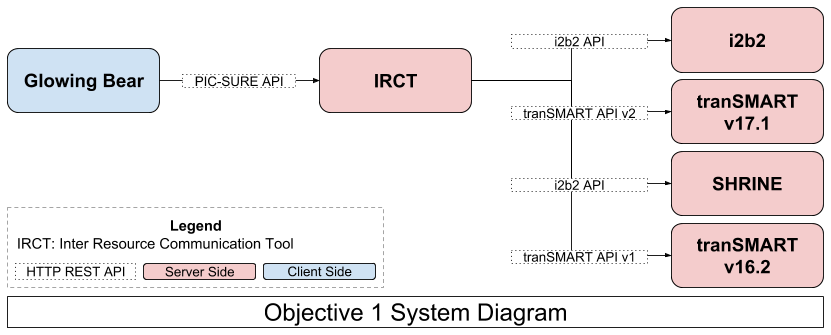
\includegraphics[width=1\textwidth]{figures/sys_diagram_obj1.png}
    \caption{System diagram of objective 1: Interoperability layer for a common front end for clinical research platforms.}
    \label{fig:sysdiagramobj1}
\end{figure}


\subsection{General Workflow}
The general workflow of the system starts in Glowing Bear.
%The users logs in using XXX TBD.
Then a specific IRCT resource is selected for the rest of the operations of this session.
The user browses the tree of entities to construct query constraints using the PIC-SURE API.
Each resource exposes this tree however it wants, but always within sticking to a common interface.
When the constraints for selecting patients are established, the user chooses what data to export.
During those last operations, the counts corresponding to the query are updated dynamically with background requests to IRCT, which itself does requests to the resources with their native API.
Finally once the full query is constructed, the user executes the final query and is able to download the results, again using one common API.


\subsection{Access Management}

The authentication is delegated to a third-party using the OpenID Connect protocol~\cite{todo}, here the third-party we use is Keycloak but it could be swapped with any software implementing the same protocol.

\begin{figure}[ht]
    \centering
    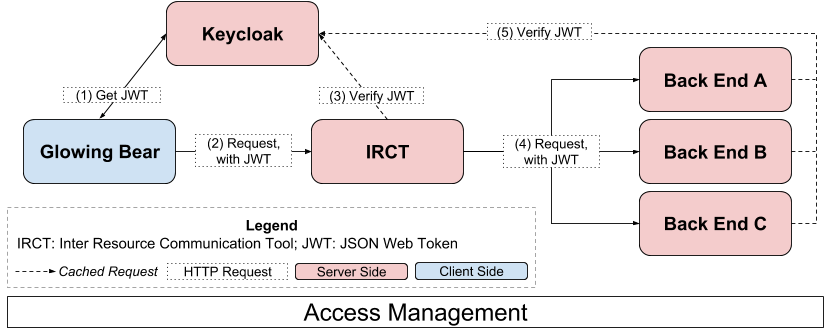
\includegraphics[width=1\textwidth]{figures/access_mgmt.png}
    \caption{Diagram of the access management design.}
    \label{fig:accessmgmt}
\end{figure}

Figure~\ref{fig:accessmgmt} shows the high-level picture of the access management in our solution, which revolves around Keycloak.
All components, i.e. IRCT and the back ends, verify the JSON Web Token embedded in the requests to authenticate the user and enforce its authorizations. %todo: cite JWT

% steps
The steps are:
\begin{enumerate}
    \item The client performs the authentication with Keycloak, with the client ID of the back end (which is set up to be the same as the IRCT resource name), and get a JSON Web Token containing the user authorizations
    \item Glowing Bear makes HTTP requests to IRCT, with the JWT embedded in the headers.
    \item IRCT verify the JWT using the public key of Keycloak. 
    The JWT contains the identifier of the signing key, which IRCT uses to requests the corresponding public key to Keycloak (and is cached to minimize the requests) and then verify the signature.
    \item The authenticated request is forwarded to the back end the user is using, the token remains the same.
    \item The back end verify the JWT using the same method as IRCT, and is responsible to enforce its own authorizations, which are contained in the JWT.
\end{enumerate}

% about client ids
Note that the JWT are verified twice in this design. 
The JWT contains the client identifier, which must be verified by the OIDC clients.
IRCT do not have its own client identifier, but verify that the identifier matches the one of the back end.
The back end has its own client identifier, and for the sake of consistency we enforce that the IRCT resource name is the same as the client identifier.

% todo: add small ccl on why this is good, and some analysis

\subsection{Glowing Bear Queries}

One of the main implementation challenge is replacing in Glowing Bear the tranSMART API v2 by the PIC-SURE API.
In Glowing Bear, all the operations the user undertakes have the objective of constructing a query to select data.
In order to give an overview of the goal of the changes in Glowing Bear, see below an example of a query with the tranSMART API v2 and its equivalent using the PIC-SURE API.
The query exports the gender for all patients aged from 20 to 25 years old in the \emph{CATEGORICAL\_VALUES} study.

\newpage
\paragraph*{tranSMART API v2 Example Query}
\begin{verbatim}
POST /export/<id>/run
{
"constraint": {
"type": "and",
"args": [
  {
    "type": "and",
    "args": [ {
      "type": "subselection", "dimension": "patient",
      "constraint": {
        "type": "and",
        "args": [
          {
            "type": "and",
            "args": [
              { "type": "concept", "conceptCode": "CV:DEM:AGE" },
              { "type": "value", "valueType": "NUMERIC", "operator": ">=", "value": 20 },
              { "type": "value", "valueType": "NUMERIC", "operator": "<=", "value": 25 }
            ]
          },
          { "type": "study_name", "studyId": "CATEGORICAL_VALUES" }
        ]
    } } ]
  }, {
    "type": "or",
    "args": [
      {
        "type": "and",
        "args": [
          { "type": "concept", "conceptCode": "CV:DEM:SEX:F" },
          { "type": "study_name", "studyId": "CATEGORICAL_VALUES" }
        ]
      }, {
        "type": "and",
        "args": [
          { "type": "concept", "conceptCode": "CV:DEM:SEX:M" },
          { "type": "study_name", "studyId": "CATEGORICAL_VALUES" }
        ]
      } ]
  }
]
},
"elements": 
  [{ "dataType": "clinical", "format": "TSV", "dataView": "default" }]
}
\end{verbatim}

\newpage
\paragraph*{PIC-SURE API Equivalent Query}
\begin{verbatim}
POST /queryService/runQuery
{
  "select": [ {
    "operation": "EXPORT",
    "fields": { "data": "clinical", "file": "TSV" }
  }, {
    "field": {
      "pui": "/<resource>/Public Studies/CATEGORICAL_VALUES/Demography/Gender/Male/",
      "dataType": "ENUM_VALUE"
    }
  }, {
    "field": {
      "pui": "/<resource>/Public Studies/CATEGORICAL_VALUES/Demography/Gender/Female/",
      "dataType": "ENUM_VALUE"
    }
  } ],
  "where": [
    {
      "field": {
        "pui": "/<resource>/Public Studies/CATEGORICAL_VALUES/Demography/Age/",
        "dataType": "INTEGER"
      },
      "predicate": "CONSTRAIN_VALUE_NUMERIC",
      "fields": { "OPERATOR": ">=", "CONSTRAINT": "20" }
    }, {
      "field": {
        "pui": "/<resource>/Public Studies/CATEGORICAL_VALUES/Demography/Age/",
        "dataType": "INTEGER"
      },
      "predicate": "CONSTRAIN_VALUE_NUMERIC",
      "fields": { "OPERATOR": "<=", "CONSTRAINT": "25" },
      "logicalOperator": "AND"
    }, {
      "field": {
        "pui": "/<resource>/Public Studies/CATEGORICAL_VALUES/",
        "dataType": "STUDY"
      },
      "predicate": "CONTAINS",
      "logicalOperator": "AND"
    } 
  ],
  "alias": "My query"
}
\end{verbatim}

We observe that the tranSMART API v2 uses a \emph{subselection} of patients to specify the constraints, and then the additional constraints (linked together by an \emph{OR}, and with the subselection by an \emph{AND}) are used to select the data to be exported.
To pursue the same objective, PIC-SURE uses \emph{where} clauses for specifying constraints and \emph{select} clauses to select the data to be exported.


\subsection{Back End Systems}

% baseline
IRCT communicates with all of the supported back end systems using their native APIs.
The compatible resources expose their tree of concept of concepts, which contain the information on how to construct queries.
They support the following basic query types, based on a specific set of constraints:
\begin{itemize}
    \item Count queries: number of matching patients
    \item Patient set queries: identifiers on matching patients
    \item Data queries: any kind of medical data about the matching patients
\end{itemize}

The constraints used can be:
\begin{itemize}
    \item Concept constraints: presence of a specific ontology item for a patient
    \item Value constraints: some numeric, text or date value satisfying some constraints
\end{itemize}

% additional features
Some features specific to some back end systems are supported only when using this system.
This is the case for systems implementing the tranSMART API v2:
\begin{itemize}
    \item Constraints based on studies / clinical trials
    \item Constraints based on pedigree / relation type
\end{itemize}

\newpage
% todo: add about transmart docker (in appendix maybe?)
% todo: explanation about data table
% todo: explanations+ modifs about transmart 16.2
% todo: integration in common interface
\section{Implementation of the Interoperability Layer}
Here is described component-per-component the implementation of the solution presented in the last section. 
Each of the sections first explains what is the current status of the relevant components, and then what needs to be modified or implemented.
First we describe the deployment of all the relevant components that need to be used in the system (refer to figure~\ref{fig:sysdiagramobj1}).
Then we are going over all the modifications made to Glowing Bear, regarding the change of the API it uses.
Finally we go over the modifications of the core of IRCT, and the implementation of all the resources it uses.


\subsection{Deploying Original Components}
% todo: transmart 16.2?
% todo: versions to be used

First of all we are compiling, setting up and deploying all the building blocks of the solution: Glowing Bear, IRCT, tranSMART 17.1, i2b2, SHRINE.
The exhaustive information about the deployments using Docker can be found in appendix~\ref{sec:docker-images}.
These components require some servers that are deployed with Docker: WildFly (application server), PostgreSQL (database server), lighttpd (web server)

% GB
We are deploying Glowing Bear from the sources using the Angular command \verb|ng serve|, which is practical for development.
For production deployment it is deployed through the web server.
The version used is branched off the development branch \verb|table|, which is the most up to date branch at the time of the writing, and is regularly rebased on this same branch.
It is configured to use the locally deployed instance of back end components.

% todo: put in annex for docker deployment, also db
Keycloak is deployed as an OpenID Connect server using its official Docker image that sets up a working instance.
It uses the same PostgreSQL database that other deployments are using.
The version used is 3.4.3.
It is configured with a local user data source managed by itself, and one client for each back end that will use this instance.

% IRCT
IRCT is compiled from sources and deployed using Docker.
The version used is a fork of the latest version on the master branch of the repository. 
It is regularly rebased to keep track of the changes.
It is configured to use one local instance of each type of supported back end systems: i2b2, tranSMART 17.1, SHRINE.
The configuration is done through the local PostgreSQL database.

% i2b2
I2b2 is compiled from sources and deployed using Docker.
The version used is TBD.
The Spring configuration files and test data comes from the demo dataset that is provided with i2b2, and allows to have a demonstration running instance, done through the local PostgreSQL database.

% tranSMART 17.1
tranSMART 17.1 is compiled from sources and deployed using Docker.
The version used is TBD.
The configuration is done through a grails configuration file, and some test data is loaded in the local PostgreSQL database used.

% SHRINE
First step of the SHRINE deployment it to modify the existing i2b2 deployment.
Its demo data (loaded in PostgreSQL) is duplicated three times, to replicate (with the appropriate configuration) three different instances of i2b2 (but served through the same web service).
Then three instances of the SHRINE web services are deployed: this corresponds to a setting where the SHRINE network has three nodes.
It is compiled from sources and deployed using Docker. 
The version used is TBD.
It is configured through simple configuration files.
The SHRINE instances use a deployment of the MySQL database server for their data.
The SHRINE webclient is served by the web server.

\subsection{Glowing Bear Modifications}
% todo: step 4 w/ data tables ?
% todo: this overview might belong in design rather than here? evaluate

% GB modif overview
Glowing Bear is pretty heavily modified, the idea being to make it a native PIC-SURE API client by replacing completely the tranSMART client API implementation. 
In general the API requests are modified through the calls in \verb|ResourceService|, and the response through the models in \verb|src/app/models/|.
On a very high-level, the important steps of the queries as mapped as such:
\begin{itemize}
    \item Step 1 (patients subselection with constraints): defining PIC-SURE \emph{where} clauses, making count queries queries with the \emph{select} clause
    \item Step 2 (selection of data to export): defining \emph{select} clauses for data export, making count queries as well
    \item Step 3 (data export): executing the export query previously built
\end{itemize}

% todo: save query is after step 2

% overview of steps taken in GB workflow: steps for modifications
The organization of this section follows Glowing Bear typical workflow:
\begin{itemize}
    \item Client initialization: loading and login
    \item Explore the tree of concepts
    \item Step 1: Construct a query or re-use a saved query
    \item Step 2: Select the data to export
    \item Save a constructed query
    \item Step 3: Export the data
\end{itemize}

% why no transmart rest v2
Compatibility with tranSMART versions 17.1+ is later restored through the implementation of an IRCT resource interface (see~\ref{sec:irct-res-transmart-17.1}).
The reasoning behind this choice is that maintaining compatibility of two different but similar APIs in Glowing Bear would be possible, but complicated, which translates into additional efforts spent on the implementation, and later on the maintenance of the code: this would be sub-optimal as these efforts are better spent elsewhere.
The potential downside of this choice is a time delay for the requests as we are introducing an additional middle-component, these are formally measured in a later chapter.%chapter~\ref{chap:perfeval}. % todo: ref


\subsubsection{Authentication \& Authorization}

IRCT uses OpenID Connect to authenticate and authorize the users of its client applications, while Glowing Bear originally implements the client side of the OAuth2 protocol for authorization with tranSMART. 
The modification to Glowing Bear is the migration from the authorization protocol OAuth2~\cite{oauth2} to the authentication and authorization protocol OpenID Connect~\cite{openidconnect}.
Since OpenID Connect is a layer on top of OAuth2, the modifications to migrate the client code from OAuth2 to OpenID Connect are not significant, and are made by making use of the \emph{angular-auth-oidc-client} library~\cite{angular-auth-oidc-client}.
The flow remains the same: Glowing Bear obtains a JSON Web Token (JWT) from the OpenID Connect provider, which will then be embedded in the header of the HTTP requests to IRCT.
These modifications are made by replacing the \verb|EndPointService| by \verb|AuthenticationService|, which implements the logic of the authentication.
Additionally a small component \verb|AutoLoginComponent| redirects to the login page of the OIDC server if the authentication token is not valid or not present.

\subsubsection{IRCT Resources Support}
% todo: summary of GB supports for predicates / operations

\paragraph{Resources List}
After the user has successfully logged in, Glowing Bear requests the list of IRCT resources available and their definitions.
Then the user chooses from the list which resource to use for the current session: it is possible to use only one resource at a time. % todo: behavior to be confirmed
The selected resource and its definition are kept in the new \verb|IRCTResourceService| service that keeps and processes all the information about the resource returned by PIC-SURE.
Among other things, this service is used to make the connection between tree data types and possible predicates that can be applied on them.
The method \verb|ResourceService.getResources()| is added to retrieve the PIC-SURE resources with the following API call:

\newpage
\begin{verbatim}
GET /resourceService/resources
\end{verbatim}

Response:
\begin{verbatim}
[
  {
    "id": 1,
    "name": "resource name (e.g. i2b2-local)",
    "implementation": "resource type (which implementation is used, e.g. i2b2XML)",
    "relationships": [ supported relationships between tree nodes, e.g. CHILD ],
    "logicaloperators": [ "AND", "OR", "NOT" ],
    "predicates": [ supported predicates and their properties, e.g.: {
        "predicateName": "predicate name (e.g. CONTAINS)",
        "displayName": "displayed name (e.g. Contains)",
        "description": "description",
        "default": true if this predicate should be selected by default,
        "fields": [ {
            "name": "field name (e.g. By Encounter)",
            "path": "field code (to be used in query, e.g. ENCOUNTER)",
            "description": "By Encounter",
            "required": true,
            "dataTypes": [ data type of the value field(s) of this predicate ],
            "permittedValues": [ permitted values, if it categorical ]
          } ],
        "dataTypes": [ data types to which this predicate applies (e.g. STRING) ],
        "paths": [ paths to which this predicate applies (empty for all) ]
      } ],
    "selectOperations": [ supported operations for select (e.g. AGGREGATE) ],
    "selectFields": [ supported fields for the operations, e.g. COUNT for AGGREGATE ],
    "joins": [ ],
    "sorts": [ ],
    "processes": [ ],
    "visualization": [ ],
    "dataTypes": [ data types and their properties, e.g.: {
        "name": "name of the data type",
        "pattern": "regex to validate the value",
        "description": "description of the data type"
    } ]
  },
  ...
]
\end{verbatim}


\paragraph{Specific Features}
\label{sec:specific-features}

\verb|IRCTResourceService| provides methods that determine if some specific features are supported, which allows some features of Glowing Bear to be enabled or disabled:
\begin{itemize}
    \item \verb|supportsCounts()|: returns \emph{true} if queries of type \verb|SELECT AGGREGATE COUNT| are supported, which enables the live counts display in the UI
    \item \verb|supportedCountsDimensions()|: if \verb|supportsCounts()| is \emph{true}, returns the countable dimensions (most commonly \emph{Patients} and \emph{Observations}).
    \item \verb|supportsNestedClauses()|: returns \emph{true} if the \emph{where} clause predicates \verb|CLAUSE_NEST| and \\
    \verb|CLAUSE_UNNEST| allowing nesting are supported
    \item \verb|supportsMinMax()| returns \emph{true} if queries of type \verb|SELECT AGGREGATE MIN/MAX| are supported
    \item \verb|supportsStudies()| / \verb|supportsClinicalTrials()|: returns \emph{true} if queries based on those specific dimensions are supported 
    \item \verb|supportsPedigrees()|: returns \emph{true} if constraints based on pedigrees are supported
    \item \verb|supportsGetTreeWithDepth()|: returns \emph{true} if the tree can be retrieved with a specified depth (if the resource declare a tree relationship as \verb|CHILDREN-DEPTH-X|)
    \item \verb|supportsDataExport()|: returns \emph{true} if data export queries are supported
\end{itemize}


\subparagraph{tranSMART Studies}

% general + into tree
The tranSMART REST API v2 has several calls that are specific to studies, while the PIC-SURE API does not have a direct equivalent to this.
However since the studies are completely embedded within the concept tree, i.e. a concept belongs to one study or it is cross-study, they can simply be abstracted into the tree of entities exposed by PIC-SURE: we create a \verb|STUDY| data type for the tree entities (see~\ref{sec:gb-tree}).
\verb|TreeNodeService.isTreeNodeAStudy()| implements the recognition of the \verb|STUDY| data type.
%todo: in model

% list of studies
If the resource supports it, \verb|ConstraintService.loadStudies()| loads the list of studies by calling \verb|ResourceService.getStudies()|, which is modified to use the following PIC-SURE call:
\begin{verbatim}
POST /queryService/runQuery
{
  "select": [ {
    "operation": "AGGREGATE",
    "fields": {
        "FUNCTION": "values",
        "DIMENSION": "study"
    }
  } ],
  "alias": "get_studies"
}
\end{verbatim}

%\subparagraph{Pedigree / Relation Type}
% todo: GB asks transmart for the relation types, but for now we are putting them into permitted values of irct definition, change that ?


\subsubsection{Concepts Tree}
\label{sec:gb-tree}
% todo: for i2b2 (when no greedy loading possible): node per node loading
% todo: this means also no constraints list (dropdown) available / also tree search
% transmart keeps the depth loading

% todo: say mechanism
% in GB: stay as currently, loading everything in background 
% in IRCT: we cache the tree (in tree service to have it once?)
% or load it during the setup?
% problem: tree may be user specific!!!
%transmart: cache is study specific, i2b2: is project specific
% from GB side: either load everything, or ndoe per node???
%from GB: ALL-CHILDREN (and not depthxx) todo
% irct: support child and all-children
%for i2b2 that will be sloow to get all nodes on the server side
% also need for step 2 the tree

% modification of request (api call)
The API call in \verb|ResourceService.getTreeNodes()| is modified according to the following:
\begin{itemize}
     \item \verb|depth| parameter is replaced by \verb|relationship|: if the resource supports the retrieval of nodes with a depth more than one, then it will be achieved through a specific entities relationship API call \verb|CHILDREN-DEPTH-X|; 
    \item parameters \verb|hasCounts| and \verb|hasTags| are removed (these fields are always returned, although can be empty according to the resource implementation)
\end{itemize}

The API request becomes:
\begin{verbatim}
GET /resourceService/path/<resource>/<path>/?relationship=<relationship>
\end{verbatim}

Response:
\begin{verbatim}
[
  {
    "pui": "/<resource>/<path>/",
    "name": "Concept internal name",
    "displayName": "Concept name",
    "description": "Concept description",
    "ontology": "Ontology Code",
    "ontologyId": "Concept ID in the ontology",
    "relationships": [ supported relationships ],
    "counts": {},
    "dataType": {
      "name": "Data type name",
      "pattern": "Validation Regex",
      "description": "Data type description"
    },
    "attributes": {
      "visualattributes": "Visual attributes",
      "customAttributeName": "customAttributeValue"
    }
  },
  ...
]
\end{verbatim}

The \verb|dataType| field allows to know which constraints defined in the resource can be applied, thus what options can be presented to the user when a query is constructed with the help of the \verb|IRCTResourceService|.
The \verb|visualattributes| field allows to modify the appearance of the concept in the UI, for example if it's a folder containing concept, or a leaf node. 
Its presence is optional so if it is absent, the appearance will stay as it is by default, this behavior is defined in the \verb|GbTreeNodesComponent| component.
The other fields can easily be mapped to original fields in Glowing Bear.

% modification relating no depth call possible
In \verb|TreeNodeService.loadTreeNodes()|, \verb|loadTreeNext()| is called to iteratively load the nodes.
\verb|loadTreeNext()| needs to be modified to account for \verb|ResourceService.getTreeNodes()| possibly not being able to load with a depth greater than one, meaning it must be called for every node of the tree.
This is determined using \verb|IRCTResourceService.supportsGetTreeWithDepth()|.
The difference between a node and a leaf is made with the use of the \verb|relationships| field: if the node supports the relationship \verb|CHILD|, it is a node for which children can be requested.

% about format of node JSON
\verb|TreeNodeService.processTreeNodes()| and \verb|processTreeNode()| process the received JSON to load it into the internal \verb|treeNodes| array containing the tree in memory, they should be adapted to fit the PIC-SURE JSON format.
This allows all the other parts of Glowing Bear that use the node to access the information needed.


\subsubsection{Query Step 1: Constraints}
% todo : concept_enum only, values are requested

% GB overall workflow for queries
The original Glowing Bear workflow for creating the constraints is the following: \\
\verb|GbConstraintComponent.onDrop()| processes the node being dropped in the query construction panel in the UI by calling \verb|ConstraintService.generateConstraintFromSelectedNode()| to generate the constraint based on the dropped node. \\
It uses \verb|ConstraintService.generateConstraintFromConstraintObject()| to construct the individual constraint objects.

The constraints generated in the step 1 of the query corresponds to the \emph{where} clauses of the PIC-SURE query: they define the criterion the resulting data must satisfy.
The components based on \verb|modules/gb-data-selection-module/constraint-component/GbConstraintComponent| and the models based on \verb|models/constraint-models/Constraint| correspond to the different PIC-SURE predicates that Glowing Bear supports.
Overall the Glowing Bear workflow stays the same at a high-level, but its implementation at the low-level undergoes significant changes to bring compatibility with PIC-SURE.

% logic
\verb|ConstraintService| is initialized with \verb|IRCTResourceService|: this allows the service to link the data types of the tree nodes with the constraints they support. \\
\verb|ConstraintService.generateConstraintFromConstraintObject()| is the core method of the constraint generation, and is thus completely re-implemented and is renamed \\
\verb|generateConstraintFromDataType()|.
It is modified to take as input the data types coming from the PIC-SURE tree, and is using the \verb|IRCTResourceService| to get the constraints corresponding to the data types, returning a \verb|Constraint| object.
\verb|generateConstraintFromSelectedNode()| is modified to have two cases only: it is a queryable node, i.e. it has a data type, or not. If it has a data type it uses \verb|generateConstraintFromDataType()| to get the constraint, if not it calls itself recursively with the children nodes.

% data types supported
\verb|generateConstraintFromDataType()| supports the following PIC-SURE data types:
\begin{itemize}
\item Primitive
    \begin{itemize}
        \item Numeric types: \verb|INTEGER|, \verb|LONG|, \verb|FLOAT|, \verb|DOUBLE|
        \item Date types: \verb|DATE|, \verb|DATETIME|
        \item String type: \verb|STRING|
    \end{itemize}

\item Custom
    \begin{itemize}
        \item Enumerated type: \verb|ENUM_FIELD| and \verb|ENUM_VALUE| (enumerated value exposed through the tree and not as a value)
        \item Ontology concept type: \verb|CONCEPT| (simple concept without value)
        \item Study: \verb|STUDY| (restrict to a specific study)
        \item Pedigree: \verb|PEDIGREE| (constraint based on relationship, e.g. parents of another selection of patients)
    \end{itemize}
\end{itemize}


\paragraph{\emph{where} Models}

% constraint models
The way the constraints are represented internally need modification, as the nature of the tranSMART constraints and the PIC-SURE \emph{where} clauses are slightly different: they are more generic, but more importantly the supported predicate for each data type are known only at the runtime.
Constraints models in \verb|src/app/models/constraint-models/| are now not based on the type of the constraint, but on the predicate used for the constraint.
The interface \verb|Constraint| remains, but the members \verb|toQueryObjectWithSubselection()|, \verb|toQueryObjectWithoutSubselection()| and \verb|parent| are removed.
The equivalent of the subselection in PIC-SURE would be the dimension, but 
\begin{enumerate*}[label=(\arabic*)]
  \item it is defined by the resources themselves,
  \item it is integrated into the \emph{select} clauses, which is handled in the second step as it is not considered a constraint;
\end{enumerate*}
justifying the removal of those members.
They also now contain data about themselves specified by the IRCT resource: predicates name, description, paths and data types it applies to, its fields (name, code, description, required flag, data type and permitted values).

% constraint models JSON generation example
\verb|toQueryObject()| takes care of generating the JSON of the constraint: all the implementing methods now needs to generate the PIC-SURE \emph{where} clauses.
Example of two different \emph{where} clauses that would be produced by the corresponding \verb|toQueryObject()| methods:
\begin{verbatim}
{
    "field": {
        "pui": "/transmart/study1/Gender/Male/",
        "dataType": "ENUM_VALUE"
    },
    "predicate": "CONTAINS"
}

{
    "field": {
        "pui": "/transmart/study1/Age/",
        "dataType": "INTEGER"
    },
    "predicate": "CONSTRAIN_VALUE_NUMERIC",
    "fields": {
        "OPERATOR": "==",
        "CONSTRAINT": "5"
    }
}
\end{verbatim}


% ----------------------------------------------------------------------------------
\paragraph{Instantiating Constraints}
\label{sec:gb-instanciating-constraints}

Because the predicates and the fields they have are known only at runtime, we create a service \verb|ConstraintFactoryService| that handles the instantiating of properly initialized \verb|Constraint| objects.
A method \verb|createConstraint()| taking as parameters the data type and and predicate returns the \verb|Constraint| object.
While some pre-defined predicates are supported by Glowing Bear (see list below), or even required for some features, not all can be supported. 
For this reason a generic \verb|Constraint| is created, that allows Glowing Bear to handle unknown constraints that resources might declare.

% list of types of constraints, based on the predicate they support
The different constraint models with their associated predicate, that together support all the PIC-SURE data types listed before, are listed below:
\begin{itemize}
    \item \verb|ConceptConstraint|: predicate \verb|CONSTRAINT_CONCEPT|, valid for \verb|ENUM_FIELD|, \verb|ENUM_VALUE|, \verb|CONCEPT| and all primitive types 
    \item \verb|FieldConstraint|: predicate \verb|CONSTRAINT_FIELD|, valid for arbitrary values of fields in dimensions (e.g. data types \verb|STUDY|, \verb|TRIAL_VISIT|), and used to create constraint based on observation date
    \item \verb|PedigreeConstraint|: predicate \verb|CONSTRAINT_PEDIGREE|, valid for pedigree data types
    \item \verb|PatientSetConstraint|: predicate \verb|CONSTRAINT_PATIENT_SET|, valid for patient set (imported through the UI)
\end{itemize}

Note that \verb|StudyConstraint| and \verb|TrialVisitConstraint| are merged within the new \verb|FieldConstraint|, similarly \verb|GbStudyConstraintComponent| into the new \verb|GbFieldConstraintComponent|.
The trial-visit logic form \verb|GbConceptConstraintComponent| is moved to \verb|GbFieldConstraintComponent|.
Note also that not all constraints are supported by all resources, the support is known by using \\
\verb|IRCTResourceService.supports*()| methods. 

\subparagraph{Concept Constraint}
This is a simple constraint based on the presence of a concept and possibly its associated value.
A change from the original behavior is the way the values of the enumerated field are recuperated: this is done through the tree by looking at the data types, enumerated fields have a \verb|ENUM_FIELD| types, and its possible values are children of the node with the type \verb|ENUM_VALUE|.
Another change concerns the aggregates values, see~\ref{sec:gb-step1-aggregates} for more information.
The supported operators are \verb|==|, \verb|<=|, \verb|>=|, \verb|<|, \verb|>|, \verb|LIKE[exact]|, \verb|LIKE[begin]|, \verb|LIKE[end]| and \verb|LIKE[contains]|.

Example of concept \emph{where} clauses:
\begin{verbatim}
{
    "where": [ {
            "field": {
                "pui": "/transmart/study1/Age/",
                "dataType": "INTEGER"
            },
            "predicate": "CONSTRAIN_CONCEPT", 
            "fields": { "OPERATOR": ">=", "VALUE":"20" } 
        }, {
            "field": {
                "pui": "/transmart/study1/Age/",
                "dataType": "INTEGER"
            },
            "predicate": "CONSTRAIN_CONCEPT", 
            "fields": { "OPERATOR": "<=", "VALUE":"25" },
            "logicalOperator": "AND"
        }, {
            "field": {
                "pui": "/transmart/study1/Gender/Male/",
                "dataType": "ENUM_VALUE"
            },
            "predicate": "CONSTRAIN_CONCEPT"
        } ]
}
\end{verbatim}

\subparagraph{Field Constraint}
This new constraint allows to restrict according to the value of field in some dimension of the data.
It allows to query for a study, clinical-trial visit, observation date, and others.
It is implemented in the constraint model \verb|FieldConstraint| and the component \verb|GbFieldConstraintComponent|.

Example of field \emph{where} clauses generated:
\begin{verbatim}
{
    "where": [ {
            "predicate": "CONSTRAIN_FIELD", 
            "fields": { 
                "DIMENSION": "study", "FIELD":"study_id", 
                "OPERATOR": "==", "VALUE": "ORACLE_1000_PATIENT" 
            } 
        }, {
            "predicate": "CONSTRAIN_FIELD", 
            "fields": { 
                "DIMENSION": "trial_visit", "FIELD":"rel_time_num", 
                "OPERATOR": "==", "VALUE": "2" 
            },
            "logicalOperator": "AND"
        }, {
            "predicate": "CONSTRAIN_FIELD", 
            "fields": { 
                "DIMENSION": "observation", "FIELD":"start_date", 
                "OPERATOR": "<=", "VALUE": "2010-02-22" 
            },
            "logicalOperator": "AND"
        } ]
}
\end{verbatim}

\subparagraph{Pedigree Constraint}
Constraints based on pedigree are special in that they are based on other constraints (e.g. getting the parents of patients aged more than 50).
We add for them a predicate \verb|CONSTRAINT_PEDIGREE|, which has three fields:
\begin{itemize}
    \item \verb|TYPE|, required: list of permitted values which are either the type of pedigree (parents of, siblings of, etc.) or the indicator of the end of the pedigree constraints \verb|CONSTRAINT_END| (see example after)
    \item \verb|BIOLOGICAL|, optional, default to \verb|BOTH|: either \verb|YES|, \verb|NO| or \verb|BOTH|
    \item \verb|SHARE_HOUSEHOLD|, optional, default to \verb|BOTH|: either \verb|YES|, \verb|NO| or \verb|BOTH|
\end{itemize}

Example of a pedigree \emph{where} clause:
\begin{verbatim}
{
    "where": [
        {"predicate": "CONSTRAINT_PEDIGREE", "fields": { 
          "TYPE": "PARENTS_OF", "BIOLOGICAL":"YES" 
        } },
        <classic constraints>..., 
        {"predicate": "CONSTRAINT_PEDIGREE", "fields": { "TYPE": "CONSTRAINT_END" } }
    ]
}
\end{verbatim}

Similarly to other constraints, the logic construction is implemented into \\
\verb|GbPedigreeConstraintComponent| and the model representing such a constraint is \verb|PedigreeConstraint|.
It is only enabled if \verb|IRCTResourceService.supportsPedigree()| determines so.

\subparagraph{Patient Set Constraint}
Through the UI, the user of Glowing Bear can import a patient set and use it as a constraint, this handled by \verb|GbPatientSetConstraintComponent| and stored into a model \verb|PatientSetConstraint|, which are modified to adapt to the PIC-SURE format.
It supports either an array of patient identifiers, or the identifier of a patient set.

Example of patient set \emph{where} clauses:
\begin{verbatim}
{
    "where": [
        {"predicate": "CONSTRAINT_PATIENT_SET", "fields": { "PATIENT_SET_ID": "52" } },
        {"predicate": "CONSTRAINT_PATIENT_SET", "fields": { 
          "PATIENT_IDS": "[2, 32, 96]" 
        } }
    ]
}
\end{verbatim}


% ----------------------------------------------------------------------------------
\paragraph{Logical Operators}
\label{sec:gb-logical-operators}

Glowing Bear supports the definition of nested inclusion criteria, with the criteria belonging to the same group being linked by a logical operator \emph{AND} or \emph{OR}.
PIC-SURE allows queries with several \emph{where} clauses and lets each resource declares the logical operators it supports to link them. 
However the link between the clauses is flat, a clause defines its relationship with the previous clause: nested queries are not possible natively with PIC-SURE, but a workaround is presented below.

For resources that support nested queries, they declare the support for the \verb|NESTING| predicate, having a field called \verb|TYPE| with the permitted values \verb|START| and \verb|END|.
By using these it is possible for resources to support nested queries, see the following example for the methodology:
Consider the following nested query constructed in Glowing Bear:
\begin{verbatim}
    ((H AND B) OR (D AND S)) AND X AND (H OR F)
\end{verbatim}
It would have the PIC-SURE query with the following \emph{where} clauses:
\begin{verbatim}
{
    "where": [
        {"predicate": "NESTING", "fields": { "type": "START" } },
        {"predicate": "NESTING", "fields": { "type": "START" } },
        { H },
        { B, "logicalOperator": "AND" },
        {"predicate": "NESTING", "fields": { "type": "END" } },
        {"predicate": "NESTING", "fields": { "type": "START" }, "logicalOperator": "OR" },
        { D },
        { S, "logicalOperator": "AND" },
        {"predicate": "NESTING", "fields": { "type": "END" } },
        {"predicate": "NESTING", "fields": { "type": "END" } },
        { X, "logicalOperator": "AND" },
        {"predicate": "NESTING", "fields": { "type": "START" }, "logicalOperator": "AND" },
        { H },
        { F, "logicalOperator": "AND" },
        {"predicate": "NESTING", "fields": { "type": "END" } }
    ]
}
\end{verbatim}

\verb|CombinationConstraint|, \verb|GbConstraintComponent| and \\
\verb|ConstraintService.generateConstraintFromConstraintObject()| are modified to...
\begin{itemize}
    \item support this construction by storing an array of \verb|Constraint|, appropriately setting their \\
    \verb|logicalOperator| fields and adding the nesting \emph{where} clauses;
    \item allowing or not the nesting of queries according to the resource capabilities.
\end{itemize}
Query nesting status is reflected in the UI by removing the \verb|add criterion| boxes for the attributes with a level equal to or lower than 1 if it is not supported.

% generation of the whole thing from outside
The method \verb|ConstraintService.generateSelectionConstraint()| is what is used by other parts of the code to generate the constraints defined in the first step in a format that fits the API call.
We rename it to \verb|generateWhereAttribute()| to fit the PIC-SURE jargon, and modify the method accordingly.
It returns a \verb|CombinationConstraint| as described in the previous paragraph.

\subparagraph{Negation}
The logical operator \verb|NOT| is at the same level as the \verb|AND| and \verb|OR|.
For this reason the resources declare all the following operators:
\begin{enumerate*}[label=(\arabic*)]
  \item \verb|AND|,
  \item \verb|OR|,
  \item \verb|NOT|,
  \item \verb|AND NOT|,
  \item \verb|OR NOT|.
\end{enumerate*}
Which allows all kinds of queries.


% ----------------------------------------------------------------------------------
\paragraph{User Interface}
When adding criterion at the step 1, the UI has to know what data type is the entity in order to know what input from the user is expected.
This behavior is implemented in the \verb|GbConstraintComponent| and its extending components.
These components are modified or removed to fit all the modifications previously described, to arrive at a state where there is one component for each of the supported predicates described section~\ref{sec:gb-instanciating-constraints}.
Additionally they use the information provided by \verb|IRCTResourceService| to:
\begin{itemize}
    \item offer to the user a list of the supported predicates to choose from,
    \item know what fields the predicate needs,
    \item enforce format of the fields input values with the regex or offer a dropdown list of permitted values, 
    \item enforce required or optional fields,
    \item display aggregates about the concept (such as the min, max, etc.).
\end{itemize}

The parent \verb|GbConstraintComponent| is modified to hold the data type of the dropped node, and allow for the switch between predicates (if multiple predicates are supported by the data type).
Then the extending components, one for each predicate (with the addition of the one for unknown predicates), are used according to the chosen predicate.

% todo: mention modifiers (but expose through tree)
% todo: create model SelectClause (for count example: fields pui, dataType, Function, dimension)
% todo: rename constraint to whereclause
% todo: these last 2 things, check with the common models they are doing currently

\subsubsection{Query Step 1: Aggregates}
\label{sec:gb-step1-aggregates}
%todo: model SelectClause

Glowing Bear does three kinds of aggregate queries: \emph{counts}, \emph{min} / \emph{max} and \emph{values}. 
\emph{Counts} queries are made when the user presses \emph{Update Counts} after modifying constraints (in step 1) or after modifying selected attributes for export (in step 2).
\emph{Min} / \emph{max} and \emph{values} queries are made when constructing constraints from the UI, to help the user the user by displaying some metadata.
The API calls and calling methods made are modified to use PIC-SURE as described below.
As support for aggregate \emph{select} calls is not mandatory for the resources, if the resource does not support it the related features are disabled (more info in section~\ref{sec:specific-features}).

\verb|ResourceService.getCounts()|, \verb|getStudies()| are merged into \verb|getAggregate()|.
This means that all the code calling those methods need to be adapted to fit the inputs and outputs of the new \verb|getAggregate()|.
This notably includes \verb|GbConceptConstraintComponent.initializeConstraints()|, \verb|QueryService.updateInclusionCounts()|, \verb|updateExclusionCounts()|, \verb|updateCounts_2()|, \\
\verb|updateConceptsAndStudiesForSubjectSet()|, \verb|ConstraintService.loadStudies()|.

\verb|getAggregate()| becomes more generic and accepts the following arguments:
\begin{itemize}
    \item \verb|aggregateType|: \emph{count}, \emph{min}, \emph{max}, \emph{values}
    \item \verb|dimension|: among the dimensions declared by the resource
    \item \verb|pui|: optionally a concept path if it is relevant for the query
    \item \verb|dataType|: data type of the \verb|pui|
\end{itemize}

% todo: mention the where clause in example
Example of PIC-SURE aggregate \emph{select} clauses:
\begin{verbatim}
POST /queryService/runQuery
{
  "select": [ {
    "field": { "pui": "/path/to/concept/", "dataType": "STRING" },
    "operation": "AGGREGATE",
    "fields": { "FUNCTION": "count",  "DIMENSION": "patient" }
  }, {
    "operation": "AGGREGATE",
    "fields": { "FUNCTION": "count", "DIMENSION": "observation" }
  }, {
    "field": { "pui": "/path/to/concept/", "dataType": "INTEGER" },
    "operation": "AGGREGATE",
    "fields": { "FUNCTION": "min" }
  }, {
    "field": { "pui": "/path/to/concept/", "dataType": "INTEGER" },
    "operation": "AGGREGATE",
    "fields": { "FUNCTION": "max" }
  }, {
    "operation": "AGGREGATE",
    "fields": { "FUNCTION": "values",  "DIMENSION": "study" }
  }  ],
  "where": [ <constraints> ],
  "alias": "<query_alias>"
}
\end{verbatim}


\subsubsection{Query Step 2: Data Selection}

% overview
In the PIC-SURE paradigm, this step is about preparing the \emph{select} statement of the query: the output for step 3 is the added \emph{select} causes to the query.
The changes in this part are minimal, as they are mainly about the modification of the resulting JSON containing the concepts the user wishes to get as a result, but they represent the same information.

% modifications
Originally this information is stored in a \verb|CombinationConstraint|, with individual constraints linked by a \verb|OR|.
Here for this purpose we are creating a new \verb|PICSURESelectAttribute| model containing the different \emph{select} clauses, which for each clause holds the path of the concept and the associated data type.
For the sake of consistency the method \verb|ConstraintService.generateProjectionConstraint()| is renamed to \verb|generateSelectAttribute()| and returns a \verb|PICSURESelectAttribute|.
Some additional minor modifications are made in the methods using this, such as \verb|QueryService.updateCounts_2()|, \verb|updateExports()| and \verb|GbExportComponent.runExportJob()|.

% example
Example of \emph{select} clauses generated during the second step:
\begin{verbatim}
"select": [ {
    "field": {
        "pui": "/<resource>/Public Studies/CATEGORICAL_VALUES/Demography/Age/",
        "dataType": "INTEGER"
    }
    }, {
    "field": {
        "pui": "/<resource>/Public Studies/CATEGORICAL_VALUES/Demography/Gender/Male/",
        "dataType": "ENUM_VALUE"
    }
    }, {
    "field": {
        "pui": "/<resource>/Public Studies/CATEGORICAL_VALUES/Demography/Gender/Female/",
        "dataType": "ENUM_VALUE"
    }
} ]
\end{verbatim}


\subsubsection{Saving a Query}
On top of modifying the \verb|Query| model to fit the PIC-SURE format, only the API calls to handle query saving need to be modified, the calling code remains the same.
The IRCT implementation to save and re-use saved queries is not complete: it is originally possible to only save queries, but not list or load them. 
See section~\ref{sec:irctsavedqueries} for the additional implementation in IRCT to add these features.

% saveQuery
In \verb|ResourceService.saveQuery()| the API request becomes:
\begin{verbatim}
POST /queryService/queries
{
    "queryName": <query_name>,
    "query": {
        <query_body>
    }
}    
\end{verbatim}

Response:
\begin{verbatim}
{
    "queryId": <query_id>
}    
\end{verbatim}

% getQueries
In  \verb|ResourceService.getQueries()| the API request becomes:
\begin{verbatim}
GET /queryService/queries
\end{verbatim}

Response:
\begin{verbatim}
{
    [
        "queryId": <query_id>,
        "queryName": <query_name>,
        "query": {
            <query_body>
        }
    ], [
        ...
    ],
    ...
}    
\end{verbatim}

% updateQuery
In  \verb|ResourceService.updateQuery()| the API request becomes:
\begin{verbatim}
PUT /queryService/queries/<query_id>
{
    "queryName": <query_name>,
    "query": {
        <query_body>
    }
}
\end{verbatim}

Response:
\begin{verbatim}
{
    "message": <status_message>
} 
\end{verbatim}

% deleteQuery
In  \verb|ResourceService.deleteQuery()| the API request becomes:
\begin{verbatim}
DELETE /queryService/queries/<query_id>
\end{verbatim}

Response:
\begin{verbatim}
{
    "message": <status_message>
} 
\end{verbatim}

% todo: restoreQuery()

\subsubsection{Query Step 3:  Data Export}

% intro / problem with pic-sure / overview of what is needed
Using data export with only the native \emph{select} and \emph{where} clauses of the PIC-SURE API reveals a bit limiting as IRCT originally supports only tabular results, i.e. a classic row-columns result.
Moreover there is no support for custom export parameters such as different types of data, only format of the result can be chosen between \emph{TABULAR} or \emph{JSON}.
On the other end, backends such as tranSMART supports elaborated parameters for getting results, which is a required features for our system.
For these reasons we are not using the native export mechanism of PIC-SURE in order to select the format of the data, but are defining a custom \emph{process} clause named \verb|EXPORT|, if the resource supports it.
Modifications in Glowing Bear to use PIC-SURE can be summarized in three points:
\begin{itemize}
    \item Get available data types and file formats for a specific query (export parameters);
    \item Submit export request;
    \item List exports and download them.
\end{itemize}

\paragraph{Available Export Parameters}

% API calls
\verb|ResourceService.getExportFileFormats()| requests to the back end the supported file formats for the exports.
\verb|getExportDataFormats()| requests to the back end the supported types of data to export, given the current query.
These two requests are merged into \verb|getExportFormats()| and the API calls are replaced by using a PIC-SURE query with specific \emph{select} clauses using the operation \verb|EXPORT|, example:
\begin{verbatim}
POST /queryService/runQuery
{
  "select": [ {
    "operation": "EXPORT",
    "fields": { "SUPPORTED_FORMATS": "[data, file]" }
  }, 
    <query_select_clauses>
  ],
  "where": [ <query_where_clauses> ],
  "alias": "<query_alias>"
} 
\end{verbatim}

% in service
\verb|QueryService.updateExports()| is modified to take into account the merging of these two methods and the result that is now represented differently.

\paragraph{Export Request}

% API calls
\verb|ResourceService.createExportJob()| and \verb|runExportJob()| that respectively create an run an export job are merged into \verb|runExportJob()|.
The call made is similar the previous, using \emph{select} clauses to specify the parameters of the export job:
\begin{verbatim}
POST /queryService/runQuery
{
  "select": [ {
    "operation": "EXPORT",
    "fields": { "data": "clinical", "file": "TSV" }
  }, {
    "operation": "EXPORT",
    "fields": { "data": "mrna", "file": "JSON" }
  }, 
    <query_select_clauses>
  ],
  "where": [ <query_where_clauses> ],
  "alias": "<query_alias>"
} 
\end{verbatim}

Note that the name of the fields match the possible values of the \verb|SUPPORTED_FORMATS| field.

% in component
\verb|GbExportComponent.runExportJob()| is modified to take into account the merging of these two methods and the result that is now represented differently.


\paragraph{Manage Exports}

% list
\verb|GbExportComponent.updateExportJobs()| takes care of refreshing the list of exports previously made by using \verb|ResourceService.getExportJobs()| to make the API request.
This API request is modified to:
\begin{verbatim}
GET /resultService/available
\end{verbatim}

% download
\verb|GbExportComponent.downloadExportJob()| take care handling the download of the file containing the exported results, and to do so it uses the API request made in \verb|ResourceService.downloadExportJob()|.
This call is modified to:
\begin{verbatim}
GET /resultService/result/<result_id>/ZIP?download=yes
\end{verbatim}

Note that before that a first call is made to get the available formats for the results, but in the case of multi-dimensional data it will always return \verb|ZIP|:
\begin{verbatim}
GET /resultService/availableFormats/<result_id>
\end{verbatim}

% todo: cancel / archive not covered
% todo: data table, using param in select EXPORT? process?


\subsection{IRCT-Related Implementation}

\subsubsection{IRCT Core Modifications}
% todo: version from github to select: which? there seem to be a new query param (commit on feb 2) only\_count, which may prove valuable for GB << important question to solve, check out a specific commit? last release is not recent enough as of now 
% todo: auth mechanism? TBD
% todo: no need for modif resources, we can access the user token from the resource (user is available as a field)

\paragraph{Saving Queries: Additional API Calls}
\label{sec:irctsavedqueries}

% rest api
The original IRCT does implement an API call to save a specific query: \verb|POST /queryService/savequery|.
However it does not provide a way to manage the existing queries.
As this is a required feature, we are adding it in the IRCT core.
We modify the class \verb|edu.harvard.hms.dbmi.bd2k.irct.cl.rest.QueryService| to add the following methods:
\begin{itemize}
    \item \verb|getQueries()|, implementing API call \verb|GET /queryService/queries|
    \item \verb|saveQuery()|, implementing API call \verb|POST /queryService/queries|
    \item \verb|deleteQuery()|, implementing API call \verb|DELETE /queryService/queries/<query_id>|
    \item \verb|updateQuery()|, implementing API call \verb|PUT /queryService/queries/<query_id>|
\end{itemize}

The mapping API calls to methods is done using JAX-RS~\cite{wiki:jaxrs}.

% controller
The class \verb|irct.controller.QueryController| that implements the logic of managing queries.
It needs to be modified so that the saved queries are associated to an user: the users should be able to manage only their own queries.

\paragraph{Data Export: Support of Additional Data Type}

% why + add type
The original IRCT supports results of following types: \verb|TABULAR|, \verb|JSON|, \verb|HTML|, \verb|IMAGE|.
Supports for types of results is represented through the enum \verb|edu.harvard.hms.dbmi.bd2k.irct.model.result.ResultDataType| and the the code that manipulates it.
The data exports in tranSMART and i2b2 gives multi-dimensional data that are not supported with this construction.
To support such results, we add an IRCT result type \verb|ZIP|.
The resources using this type declare it through their \verb|irct.model.resource.implementation.| \\
\verb|QueryResourceImplementationInterface.getQueryDataType()| method.

% things to modify as consequence for added type
In the newly created package \verb|irct.model.result.zip| we create a new class that implement the \verb|ZIP| result type, to do do it implements the classes
\verb|irct.model.result.Data| and \\
\verb|irct.model.result.Persistable|.
This is a pretty simple implementation that only stores the resulting files from resources on the file system.

\paragraph{Authentication Modifications}
TBD: modifications to support the authentication design
% todo


\subsubsection{IRCT Resources Implementation}

% overview
The IRCT resources needs to define two things:
\begin{itemize}
    \item declaration of its parameters and the kind of requests it supports, through SQL statements loaded in the database (we are using PostgreSQL);
    \item a Java class implementing some interfaces in a way that match the declaration of the resource capabilities.
\end{itemize}

Some of these things are already existent, but needs modifications, and some others need to be implemented from scratch.
The details of this is explained in the following paragraphs.

% java interfaces
The interfaces that are to be implemented by the resources are the following:
\begin{itemize}
    \item \verb|ResourceImplementationInterface|: generic resource, provides methods for setup and type of resource
    \item \verb|PathResourceImplementationInterface|: methods for traversing tree exposed by the resource
    \item \verb|QueryResourceImplementationInterface|: methods for running queries
    % \item \verb|ProcessResourceImplementationInterface|: methods for running processes
\end{itemize}

\paragraph{i2b2}
The i2b2 resource implementation exists in the original IRCT, along with a library that allows to communicate with i2b2.
However this implementation is not exactly adapted for our goal and needs modifications.

We make the i2b2 resource declare the following \emph{select} operations:
\begin{itemize}
    \item \verb|AGGREGATE|, fields:
    \begin{itemize}
        \item \verb|FUNCTION|, mandatory, possible values:
        \verb|COUNT|
        
        \item \verb|DIMENSION|, optional, possible values:
        \verb|observation|,
        \verb|patient|
    \end{itemize}
    
    \item \verb|EXPORT|, fields:
    \begin{itemize}
        \item \verb|SUPPORTED_FORMATS|: possible values: \verb|file| %, \verb|data|
        \item \verb|file|: value among the ones returns with \verb|SUPPORTED_FORMAT|
    \end{itemize}
    
    \item (without predicate): select data to export
\end{itemize}

And the following \emph{where} predicates:
\begin{itemize}
    \item \verb|CONSTRAIN_CONCEPT|, constraint based on a concept, field:
    \verb|OPERATOR|, optional, possible values:
    \begin{itemize}
        \item numeric values: \verb|==|, \verb|<=|, \verb|>=|, \verb|<|, \verb|>|
        \item string values: \verb|LIKE[exact]|, \verb|LIKE[begin]|, \verb|LIKE[end]|, \verb|LIKE[contains]|
    \end{itemize}
    
    \item \verb|CONSTRAINT_PATIENT_SET|, constraint based on a patient set, fields:
    \begin{itemize}
        \item \verb|PATIENT_SET_ID|: identifier of a patient set stored in the back end
        \item \verb|PATIENT_IDS|: array of patient identifiers
    \end{itemize}
\end{itemize}

% tree
Browsing the i2b2 tree of concepts if already implemented and does not need modification, except from the visual attributes parameters that is adapted to fit with a common standard.

% queries: select / where
The modifications are mainly targeted at fitting the exposed \emph{where} predicates and \emph{select} operations.
However there is a larger modification, which is to adapt the parsing of the \emph{AND} / \emph{OR} queries as described section~\ref{sec:gb-logical-operators} as they need to be re-organized in the resource implementation to fit the native i2b2 way of querying, which has a non flexible syntax:
\begin{verbatim}
    (A OR B OR ...) AND (X OR Y OR ...) AND ...
\end{verbatim}
Note that the i2b2 resource does not support query nesting.

% i2b2 parse and or:
% Y OR Z OR (A AND B)
% (Y OR Z OR A) AND (Y OR Z OR B)

\paragraph{tranSMART 17.1}
\label{sec:irct-res-transmart-17.1}

We make the tranSMART 17.1 resource declare the following \emph{select} operations:
\begin{itemize}
    \item \verb|AGGREGATE|, fields:
    \begin{itemize}
        \item \verb|FUNCTION|, mandatory, possible values:
        \verb|COUNT|,
        \verb|MIN|,
        \verb|MAX|,
        \verb|VALUES|
        
        \item \verb|DIMENSION|, optional, possible values:
        \verb|observation|,
        \verb|patient|,
        \verb|study|,
        \verb|trial_visit|
    \end{itemize}
    
    \item \verb|EXPORT|, fields:
    \begin{itemize}
        \item \verb|SUPPORTED_FORMATS|: possible values: \verb|file|, \verb|data|
        \item \verb|file|: value among the ones returns with \verb|SUPPORTED_FORMAT|
    \end{itemize}
    
    \item (without predicate): select data to export
\end{itemize}

And the following \emph{where} predicates:
\begin{itemize}
    \item \verb|CONSTRAIN_CONCEPT|, constraint based on a concept, field:
    \verb|OPERATOR|, optional, possible values:
    \begin{itemize}
        \item numeric values: \verb|==|, \verb|<=|, \verb|>=|, \verb|<|, \verb|>|
        \item string values: \verb|LIKE[exact]|, \verb|LIKE[begin]|, \verb|LIKE[end]|, \verb|LIKE[contains]|
    \end{itemize}

    \item \verb|CONSTRAIN_FIELD|, constraint based on a field in one of the dimension, fields:
    \begin{itemize}
        \item \verb|DIMENSION|
        \item \verb|FIELD|
        \item \verb|OPERATOR|
        \item \verb|VALUE|
    \end{itemize}
    
    \item \verb|CONSTRAIN_PEDIGREE|, constraint based on relationship between patients, fields:
    \begin{itemize}
        \item \verb|TYPE|, e.g. \verb|PARENTS_OF|, etc. among permitted values
        \item \verb|BIOLOGICAL|, possible values: \verb|YES|, \verb|NO|, \verb|BOTH|
        \item \verb|CONSTRAINT_END|
    \end{itemize}
    
    \item \verb|CONSTRAINT_PATIENT_SET|, constraint based on a patient set, fields:
    \begin{itemize}
        \item \verb|PATIENT_SET_ID|: identifier of a patient set stored in the back end
        \item \verb|PATIENT_IDS|: array of patient identifiers
    \end{itemize}
    
    \item \verb|NESTING|, fields: \verb|TYPE| (values: \verb|start| or \verb|end|)
    
\end{itemize}

% lib
First in order to support all the calls to tranSMART 17.1 backends that are needed, a simple client library for tranSMART REST API v2 is developed.
In terms of features, this library offers all calls that were previously available in Glowing Bear, and that will be used to answer the calls from the PIC-SURE API.

% tree
The tree exposed through the PIC-SURE API is the same as the tranSMART 17.1.
Natively PIC-SURE does not support browsing the tree at more than one level at a time, so we add another relationship supported in browsing the tree: \verb|CHILDREN-DEPTH-X|, that will return children with a depth up to \verb|X|.
The visual attributes parameters is added in order to display with the proper type in the UI the node, an example of this is the study: it is a \verb|STUDY| node in the tree, and in order to be displayed as such in the UI the visual attributes parameters is set as such.

% queries: select / where
All the predicates and operations described before are translated into the native API in a straightforward way, as all the information for input is available.
The is a special case: if the queried concept belongs to a study, a study constraint is added, while if the concept is cross-study it is left as is.
The nesting of queries described section~\ref{sec:gb-logical-operators} is implemented in the resource and translated in the native API.

%todo: construction of query: need to fetch in tree the constraint to be used

\paragraph{SHRINE}
The SHRINE API is basically a limited i2b2 API (saves for some very minor additional fields).
It supports only counts, which means no data exports.
The only significant difference is in the results, as one query brings several results.
We take the i2b2 implementation and slightly modify to the purpose of being compatible with SHRINE nodes.

The resource exposes the following \emph{select} operations:
\begin{itemize}
    \item \verb|AGGREGATE|, fields:
    \begin{itemize}
        \item \verb|FUNCTION|, mandatory, possible values:
        \verb|COUNT|
        
        \item \verb|DIMENSION|, optional, possible values:
        \verb|observation|,
        \verb|patient|
    \end{itemize}
\end{itemize}

And the following \emph{where} predicates:
\begin{itemize}
    \item \verb|CONSTRAIN_CONCEPT|, constraint based on a concept, field:
    \verb|OPERATOR|, optional, possible values:
    \begin{itemize}
        \item numeric values: \verb|==|, \verb|<=|, \verb|>=|, \verb|<|, \verb|>|
        \item string values: \verb|LIKE[exact]|, \verb|LIKE[begin]|, \verb|LIKE[end]|, \verb|LIKE[contains]|
    \end{itemize}
\end{itemize}

%todo: \paragraph{tranSMART 16.2} it is not tranSMART 16.2 :( but i2b2 transmart

\subsection{Back Ends Modifications}
\subsubsection{i2b2 \& derivatives}
% todo: class to be implemented i saw about: https://github.com/i2b2/i2b2-core-server/tree/master/edu.harvard.i2b2.pm/src/edu/harvard/i2b2/pm/util
TBD: modify PM to support OIDC (will support medco and shrine as well)
add impl. for check token, considered as a simple pw
elaborate on this subject
set istoken to true
SessionKey: is the tag for i2b2 session
user mgmt?

\subsubsection{tranSMART 17.1}
% todo
TBD: using spring security, get OIDC compatibility
authorizations?


% todo: CHILD_DEPTH: how it works (decided server side, incremental, etc.)
% todo: implementation specifics, i2b2 cache, only project/categories level
% todo: i2b2 modifiers: todo
% i2b2: not possible to query 2 projects at same time
\chapter{Privacy-Preserving Cohort Exploration}
\label{sec:medco}


% thesis: medco subject to previous work of author, modified as such... (check out paper for more info)

% intro
% We adapt and integrate a privacy-pres
% Building on top of the interoperability layer described in the last section, we achieve in this section the ability to do cohort exploration with our system in a privacy-preserving way.

% explain what is medco, several nodes, etc.
\section{Detailed Workflow}

We show here the detailed workflow of our system when using MedCo.
The first two step \ref{enum:wf-interop-login} and \ref{enum:wf-interop-login} from the interoperability layer (section~\ref{sec:interoplayer-wf}) are the same, and the following differs:

\begin{enumerate}
\item \textbf{User Login}:
T

\end{enumerate}

% todo: put medco more detailed diagram

\begin{itemize}
\item \textbf{Query Construction}:
The user browses the tree of query terms and uses them to construct a query corresponding to a patient set.
When adding a term into the query panel, Glowing Bear might, according to its type, make a background request to fetch the term metadata, which is the case for example for categorical or numerical terms.
The user then optionally sets value(s) to the query term.

\end{itemize}

mention about edco resource ahs to be implemented: in two parts mainly: tree and querhy

result is same as i2b2
tree is same as i2b2 almost / converter for types added

medco builds on i2b2, as a cell in hive 

uses i2b2 api with some fine tuning 
(result in json show it 
encrypted key show it

medco cell processing show it : encrypted -> tagged)

\section{Glowing Bear Query Construction}
say it is inherated from i2b2 / 
data types new
% assumptions made:
% - ontologies match exactly
% - authentication: user exists in the 3 pms?


% for implementation of medco res. interface / extends though

\begin{itemize}
    \item tree browsing, number to encrypt in the tree
    \item same as described before, with a special data type and predicate used
    \item encryption of terms 
    \item format of encrypted terms
\end{itemize}

% gen temporary priv / pub pair of keys for user, in impl: hardcoded
% encrypt with group.toml file from config the values to be sent
% decrypt w/ priv key the results

\subsection*{Implementation}

- npm package
- key gen


\section{IRCT Query Broadcast}

% intro
After Glowing has submitted to IRCT the query through the PIC-SURE API, IRCT invokes the MedCo data source implementation to run the query with the MedCo nodes.
Running the query with the MedCo nodes uses the i2b2 XML API, but do not reuse the i2b2 data source implementation like with the tree browsing, due to fundamental differences in how the query is executed.

% threading
The process to generate the query in the i2b2 XML API format is the same as i2b2, described section~\ref{sec:interop-layer-query-translation}, even though the paths of the queried items are encrypted values.
However the submission of the query to i2b2 is different, as the query has to be submitted to all the MedCo nodes simultaneously.
This is needed as the MedCo nodes later need to synchronize between to perform some collective cryptographic operations.


% medco resource, where? should be before

\subsection*{Implementation}

% threading
We implement the part of the PIC-SURE data source implementation for MedCo that handles the querying of the data source.
To implement the simultaneous querying of the MedCo nodes, we use as many threads as there are nodes and execute them at the same time. 
We use a \emph{count down latch} to synchronize the threads together and wait on their completion.
After a set amount of time without answer from the MedCo nodes, they timeout.

% shrine drop
The query is submitted directly to the MedCo nodes. 
This is different from the original MedCo behavior that relies on SHRINE~\cite{todo} to do so.
In this previous implementation, the query was submitted to a single SHRINE node, and only after the query was broadcasted to the MedCo nodes.
Here this broadcaster role is taken by the PIC-SURE data source implementation of MedCo.
The reasoning bypassing SHRINE is that it is a multi-components software, that is complicated to set up and deploy, and is expensive to maintain.
Moreover it was not bringing a significant added value to MedCo.

% ontology
Doing so, we lose a feature offered by SHRINE, which is the ontology translation that SHRINE operates, between a common network ontology and a local i2b2 ontology.
This is not a big problem, as anyway the mapping between the network and common ontology needed to be made and maintain manually in SHRINE.
Also this feature is not used in MedCo for the encrypted terms.
It implies though that the ontologies between the different MedCo nodes have to be maintained identical, at least for the ontologies meant to be queried through MedCo.

\section{MedCo Query Processing}
\begin{itemize}
    \item summarize how medco works
    \item modifications made: shrine drop, ?
\end{itemize}

secure shuffle with aaaaaaa

% each ontologiy at each site has 2 ontologies, clear and not clear, explorable by client or not 
% schemas "medcon otology" " i2b2metadata_i2b2"


% no repeat of what medco process is doing and already described in paper, cite it in detail though


\section{Glowing Bear Result Processing}

% intro
Following the same process as i2b2 described in section~\ref{sec:interoplayer-gb-results}, the results of the query are retrieved from IRCT.
The difference here is in the format of the results, as they are encrypted with the public key $P_k$ sent along the query.

% result format
There is one result per MedCo nodes.
According to access level of the user, it is possible to identify which result is coming from which node, or the result were securely shuffled between the nodes.
The format of the result is a JSON string with the following format:

\begin{verbatim}
{
    "pub_key": "<public key used>",
    "enc_count_result": "<result encrypted with public key>",
    "times": {
        <breakdown of time measurements>
    }
}    
\end{verbatim}

% decryption
All the encrypted results are then decrypted using the secret private key $p_k$, summed together, and displayed to the user using the same process as for i2b2.
Additional information, containing the more detailed breakdown of results per node, is also displayed.


\subsection*{Implementation}

% decryption
A modification is made in the Glowing Bear PIC-SURE results processing to identify correctly when encrypted results are fetched, and extract them.
Decryption of the results are made using the cryptography library previously described, and the private key corresponding to the public key used.

% breakdown component
A new module is implemented in order to display the detailed breakdown of the MedCo query.
It appears as a tab when Glowing Bear detects the presence of MedCo results, and displays the count breakdowns and times measurements from the nodes.

\chapter{System Evaluation}

% todo: this section should show how the requirements are met

\begin{itemize}
    \item goals: meet the requirements
\end{itemize}

\section{Experiments}
% todo: overhead compared to orig GB

% - questions to be answered: overhead of this new implementation + security of the whole system
% - exp. setup
% - experiments
% - summary

\begin{itemize}
    \item i2b2 query times vs picsure+i2b2 query times (overhead)
    \item medco query times with pic-sure vs previously with shrine (refer to the paper)
    \item experimental setup & methodology
\end{itemize}

% put that or not? see if there is sth to say
\section{Security Analysis}
\begin{itemize}
    \item security analysis
    \item threat model
\end{itemize}

% - : i2b2 pws in clear in xml changed 
% where are other problems?
% how to do an analysis: cehck out owasp?
% threats models: https://www.owasp.org/index.php/Testing_Guide_Introduction#Threat_Modeling
% https://www.owasp.org/images/1/19/OTGv4.pdf ?

% (incl. medco threat model in there)
% have zones for data and such
% including communications, systems

% authorizations

% need for https comms (proxied here)


\section{Requirements Fulfillment}
\begin{itemize}
    \item take list of requirements and explain how they are met
\end{itemize}

\section{Discussion}
\begin{itemize}
    \item limitations
\end{itemize}

\chapter{Conclusion}
% not just summary: insightful conclusion

\section{Future Work}

\begin{itemize}
    \item additional pic-sure resources: HAIL, ODSY OMOP
    \item for HAIL: the R connector through PIC-SURE, work of Denise
    \item missing features: query saving, data extraction
\end{itemize}

% HAIL / R / PIC-SURE: https://www.ncbi.nlm.nih.gov/pubmed/29267850
% checkout/mention more general systems: scidb / elasticsearch / olap-mdx (mdx is the query language, olap the model)-could be envisioned to be supported thorgh pic sure --> go to future work

% add blockchain auth (gb)

% ---- appendices ----
\newpage
\appendix
%\chapter{Implementation Timeline}
\section{Overall Planning}

\begin{figure}[h!]
    \centering
    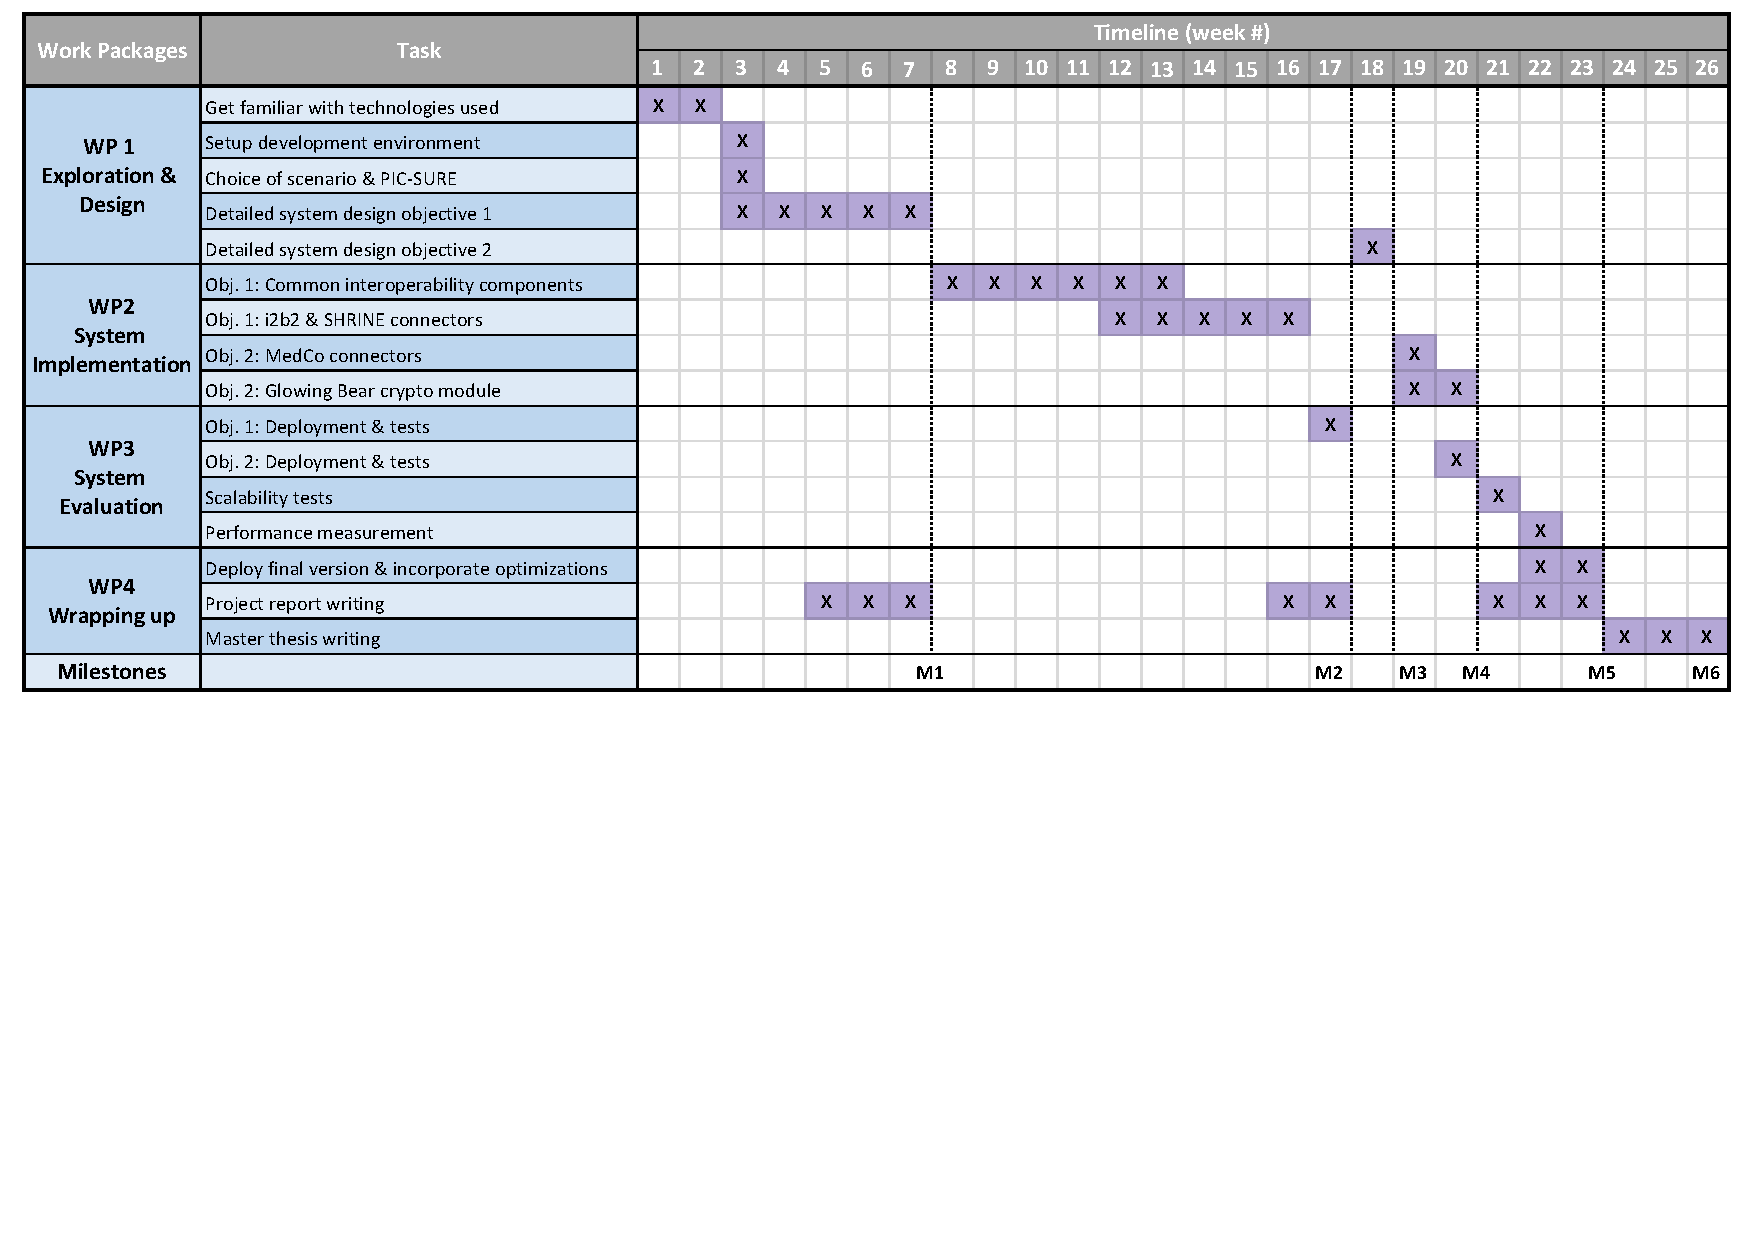
\includegraphics[width=1\textwidth,trim={0 9cm 0 0},clip]{figures/gantt_chartt_v2.pdf}
    \caption{Gantt Chart of Planning v2 (updated at M1)}
    \label{fig:overallplanning}
\end{figure}


\section{Objective 1: Interoperability Layer}

The timeline aims to have first a working system with Glowing Bear, IRCT and i2b2 by taking an horizontal approach, i.e. have each feature working end-to-end individually.
Then the different resources are made to be working with the system.
Total of the implementation of objective 1 is 10 weeks: 9 weeks are detailed in the breakdown, and an additional week as margin of error.

\begin{itemize}
    \item System initialization (login, resource list, etc.): \emph{1w}
    \begin{itemize}
        \item Setup: i2b2 + IRCT deployment
        \item IRCT resource: i2b2 resource declaration
        \item Glowing Bear: \verb|IRCTResourceService|, configuration
        \item IRCT: ??  TBD: Authentication % TODO
    \end{itemize}
    
    \item Concepts Tree: \emph{1w}
    \begin{itemize}
        \item Glowing Bear: PIC-SURE modifications
        \item IRCT resource: i2b2 tree browsing
    \end{itemize}
    
    \item Query Step 1: Constraints and Aggregates: \emph{2w}
    \begin{itemize}
        \item Glowing Bear: \emph{where} clauses construction
        \item IRCT resource: i2b2 constraints
        \item Glowing Bear: aggregate queries
        \item IRCT resource: i2b2 aggregate queries
    \end{itemize}
    
    % todo: rename data selection to variables selection
    \item Query Step 2: Variables Selection: \emph{0.5w}
    \begin{itemize}
        \item Glowing Bear: \emph{select} clauses construction
        \item IRCT resource: i2b2 variables selection
    \end{itemize}
    
    \item Query Saving: \emph{0.5w}
    \begin{itemize}
        \item IRCT core modification: add missing API calls
        \item IRCT core modification: query per user
        \item Glowing Bear: PIC-SURE modifications
    \end{itemize}
    
    \item Query Step 3: Data Export: \emph{1w}
    \begin{itemize}
        \item Glowing Bear: PIC-SURE modifications
        \item IRCT core modification: add zip file type
        \item IRCT resource: i2b2 result export
    \end{itemize}

    \item IRCT resource: tranSMART 17.1: \emph{2w}
    \begin{itemize}
        \item Setup: tranSMART 17.1 deployment
        \item Concepts tree browsing
        \item Constraints and Aggregates
        \item Variables selection
        \item Data export
    \end{itemize}
    
    \item IRCT resource: SHRINE: \emph{1w}
    \begin{itemize}
        \item Setup: SHRINE deployment
        \item IRCT resource: extend i2b2, make SHRINE-specific modifications
    \end{itemize}
\end{itemize}

% todo: acronyms in appendix
\chapter{Docker-Based Testing Infrastructure}
\label{sec:docker}

% This appendix describes the docker-based infrastructure put in place to test the systems.

\section{Docker Images}
\label{sec:docker-images}


% \subsection{Deploying Original Components}
% % todo: transmart 16.2?
% % todo: versions to be used

% First of all we are compiling, setting up and deploying all the building blocks of the solution: Glowing Bear, IRCT, tranSMART 17.1, i2b2, SHRINE.
% The exhaustive information about the deployments using Docker can be found in appendix~\ref{sec:docker-images}.
% These components require some servers that are deployed with Docker: WildFly (application server), PostgreSQL (database server), lighttpd (web server)

% % GB
% We are deploying Glowing Bear from the sources using the Angular command \verb|ng serve|, which is practical for development.
% For production deployment it is deployed through the web server.
% The version used is branched off the development branch \verb|table|, which is the most up to date branch at the time of the writing, and is regularly rebased on this same branch.
% It is configured to use the locally deployed instance of back end components.

% % todo: put in annex for docker deployment, also db
% Keycloak is deployed as an OpenID Connect server using its official Docker image that sets up a working instance.
% It uses the same PostgreSQL database that other deployments are using.
% The version used is 3.4.3.
% It is configured with a local user data source managed by itself, and one client for each back end that will use this instance.

% % IRCT
% IRCT is compiled from sources and deployed using Docker.
% The version used is a fork of the latest version on the master branch of the repository. 
% It is regularly rebased to keep track of the changes.
% It is configured to use one local instance of each type of supported back end systems: i2b2, tranSMART 17.1, SHRINE.
% The configuration is done through the local PostgreSQL database.

% % i2b2
% I2b2 is compiled from sources and deployed using Docker.
% The version used is TBD.
% The Spring configuration files and test data comes from the demo dataset that is provided with i2b2, and allows to have a demonstration running instance, done through the local PostgreSQL database.

% % tranSMART 17.1
% tranSMART 17.1 is compiled from sources and deployed using Docker.
% The version used is TBD.
% The configuration is done through a grails configuration file, and some test data is loaded in the local PostgreSQL database used.

% % SHRINE
% First step of the SHRINE deployment it to modify the existing i2b2 deployment.
% Its demo data (loaded in PostgreSQL) is duplicated three times, to replicate (with the appropriate configuration) three different instances of i2b2 (but served through the same web service).
% Then three instances of the SHRINE web services are deployed: this corresponds to a setting where the SHRINE network has three nodes.
% It is compiled from sources and deployed using Docker. 
% The version used is TBD.
% It is configured through simple configuration files.
% The SHRINE instances use a deployment of the MySQL database server for their data.
% The SHRINE webclient is served by the web server.


%mention keycloak + postgresql, not from scratch images

\subsection{i2b2}

\subsection{tranSMART 17.1}

\subsection{IRCT}

\subsection{i2b2 MedCo}
% todo: medco docker create ont schema medco


% This section describes the different Docker images of the infrastructure.

% \subsection{WildFly Application Server}

% \begin{itemize}
%     \item Ports exposed
%         \begin{itemize}
%         \item 8080: deployments endpoint
%         \item 9990: WildFly management interface
%         \end{itemize}
        
%     \item Volumes
%         \begin{itemize}
%         \item \verb|/opt/jboss/wildfly/standalone/deployments/|: deployment folder of WildFly
%         \item \verb|/opt/jboss/wildfly/standalone/configuration/|: configuration folder of WildFly
%         \item \verb|/opt/jboss/.grails/|: Grails configuration folder (for user \verb|jboss|)
%         \end{itemize}
% \end{itemize}

% This sets up a working WildFly server and install several tools used to build from source the different WARs that are deployed.
% Upon initial creation of the container there is no deployment, they are built on demand with the help of the build scripts that are shipped in the image.
% With the container running, run the following command to build a deployment: 

% \begin{verbatim}
% docker exec -it <container_name> build-war.sh <deployment_name>
% \end{verbatim}

% When running with the default docker-compose configuration, the name of the container would be \verb|deployments_wildfly-server_1|.
% Below are described the different deployments that can be built.

% \subsubsection{i2b2}
% Deployment name: \verb|i2b2|, URL exposed: \verb|/i2b2/|

% The i2b2 WAR is actually a deployment of Axis2. Within this deployment, all the i2b2 cells are deployed as AAR files (Axis2 Archive):

% \begin{itemize}
%     \item \verb|CRC|: Clinical Research Chart (data repository)
%     \item \verb|ONT|: Ontology management
%     \item \verb|PM|: Project Management (authentication and authorization)
%     \item \verb|WORK|: Workflow management (query, result sharing)
%     \item \verb|FR|: File Repository
%     \item \verb|IM|: Identity Management
% \end{itemize}

% \subsubsection{IRCT}
% Deployment name: \verb|irct|, URL exposed: \verb|/IRCT-CL/|

% Note that before you can build the IRCT deployment, i2b2 should have been built before (in order to deploy the JDBC drivers), and the database should up and initialized correctly.
% This is due to the fact that IRCT uses Hibernate to handle its data storage in the database, and when ran it will validate and update if necessary the database schema.
% To resolve an incompatibility of IRCT using Hibernate with the use of PostgreSQL, Hibernate is configured to add a prefix to all of the tables.

% \subsubsection{tranSMART 17.1}
% Deployment name: \verb|transmart-17.1|, URL exposed: \verb|/transmart-17.1/|

% % todo: a few lines


% % todo: deployments to add: tranSMART 16.2, SHRINE, MedCo

% \subsection{PostgreSQL Database Server}

% \begin{itemize}
%     \item Ports exposed
%         \begin{itemize}
%         \item 5432: PostgreSQL port
%         \end{itemize}
        
%     \item Volumes
%         \begin{itemize}
%         \item \verb|/var/lib/postgresql/data/|: PostgreSQL database files
%         \end{itemize}
% \end{itemize}

% This sets up a working PostgreSQL server and install several tools needed by the loading scripts that are ran upon the first run of the container.
% These scripts are copied in the \verb|/docker-entrypoint-initdb.d| folder.

% Below is an overview of the databases created.

% \subsubsection{i2b2}
% Contains the i2b2 database schemas for all the cells and the default demo data.

% \subsubsection{irct}
% Contains a snapshot of the IRCT database structure (that is updated as needed by Hibernate), and the resources information used by IRCT to connect to the resources:

% \begin{itemize}
%     \item \verb|i2b2-local|: the local i2b2 instance
% \end{itemize}

% \subsubsection{transmart\_17\_1}
% Contains the structure and some default test data for tranSMART 17.1.
    
\subsection{Lighttpd Web Server}

% \begin{itemize}
%     \item Ports exposed
%         \begin{itemize}
%         \item 80: HTTP port
%         \end{itemize}
% \end{itemize}

% This sets up a working Lighttpd server with PHP and install several services:
% \begin{itemize}
%     \item \verb|/phppgadmin/|: phpPgAdmin PostgreSQL management tool
%     \item \verb|/i2b2-client/|: the i2b2 webclient, using the local i2b2 instance
%     \item \verb|/i2b2-admin/|: the i2b2 admin tool, managing the local i2b2 instance
% \end{itemize}


\section{Docker-Compose Run Configuration}
% A default \verb|docker-compose.yml| is provided and works out of the box to create and deploy the images described section~\ref{sec:docker-images}.
% It creates a network to allow all the containers to communicate, exposes on the host the same ports as exposed by the container, and maps the WildFly volumes to directories alongside the Dockerfile.
% It does not require additional argument to be built and upped with the default configuration.

\chapter{APIs Usage Examples}

This appendix gives examples on how to use some APIs that are referred to in the thesis.

\section{tranSMART REST API v2}

% todo: make better and more
% todo: contains REAL examples (i.e. real response)
\paragraph{List of studies}
The list of available studies is requested:
\begin{verbatim}
GET /v2/studies
\end{verbatim}

Response:
\begin{verbatim}
{
  "studies": 
  [
    {
      "id": -20,
      "studyId": "CATEGORICAL_VALUES",
      "bioExperimentId": -10,
      "dimensions": 
      [
        "concept",
        "patient",
        "study"
      ]
    },
    ...
}
\end{verbatim}

\paragraph{Query Terms Tree}
The tree of the queryable terms is recuperated, with a depth of 2:
\begin{verbatim}
GET /v2/tree_nodes?root=&depth=2&tags=true
\end{verbatim}

Response:
\begin{verbatim}
{
  "tree_nodes":
    [
      {
        "name":"Vital Signs",
        "fullName":"\Vital Signs\",
        "name":"Vital Signs",
        "type":"UNKNOWN",
        "visualAttributes": ["FOLDER","ACTIVE"], 
        "children": [
          {
            "name":"Heart Rate",
            "fullName":"\Vital Signs\Heart Rate\",
            "conceptCode":"VSIGN:HR",
            "conceptPath":"\Vital Signs\Heart Rate\",
            "name":"Heart Rate",
            "type":"NUMERIC",
            "visualAttributes":["LEAF","ACTIVE","NUMERICAL"],
            "constraint": {
              "type": "concept",
              "conceptCode": "VSIGN:HR"
            }
          }
        ]
      },
      ...
    ]
}
\end{verbatim}

\paragraph{Saved Queries}
The list of previously saved queries is retrieved:
\begin{verbatim}
GET /v2/queries
\end{verbatim}

Response:
\begin{verbatim}
{
  "id": 1,
  "name": "testquery",
  "patientsQuery": {
    "constraint": {
      "args": 
      [
        {
          "conceptCode": "birthdate",
          "conceptPath": "\Demographics\Birth Date\",
          "fullName": "\Projects\Survey 1\Demographics\Birth Date\",
          "name": "Birth Date",
          "type": "concept",
          "valueType": "DATE"
        },
        {
          "studyId": "SURVEY1",
          "type": "study_name"
        }
      ],
      "type": "and"
    },
    "dimension": "patient",
    "type": "subselection"
  },
  "observationsQuery": {
    "data": [ ]
  },
  "apiVersion": "2.0",
  "bookmarked": false,
  "createDate": "2018-03-11T15:30:07Z",
  "updateDate": "2018-03-11T15:30:07Z"
}
\end{verbatim}


\paragraph{Query}

\begin{verbatim}
POST /v2/observations/counts_per_study_and_concept

{
  "constraint": {
    "type": "or",
    "args": [
      {
        "type": "subselection",
        "dimension": "patient",
        "constraint": {
          "type": "and",
          "args": [
            {
              "type": "concept",
              "conceptCode": "birthdate"
            },
            {
              "type": "study_name",
              "studyId": "SURVEY1"
            }
          ]
        }
      },
      {
        "type": "subselection",
        "dimension": "patient",
        "constraint": {
          "type": "and",
          "args": [
            {
              "type": "concept",
              "conceptCode": "O1KP:CAT1"
            },
            {
              "type": "study_name",
              "studyId": "ORACLE_1000_PATIENT"
            }
          ]
        }
      }
    ]
  }
}
\end{verbatim}

\subsection{Glowing Bear Workflow}
calls:
--- init step 0
1. /studies: list of studies, displayed under "Public Studies", some under "Private Studies" (distinction how??), and more, but how exactly are they mapped to the tree?

2. --> they are mapped with call to /tree\_nodes?root=\\ => each of the concept has a studyId to do the mapping
--> call to /tree\_nodes has also parameters depth --> IRCT only has depth 1, tree traversal in UI might need modifs

3. /queries: list of saved queries returned

4. /jobs: export jobs (running or not) --> not sure how IRCT handles that -> investigate / might need a change

5. /counts\_per\_study\_and\_concept: return counts for all studies / sub things -> see if how to map to irct, either as data or as process?

6. /counts: with param true, to display the total counts available

--- query step 1
7. /aggregates\_per\_concept : metadata of the concept, to display min max count etc. (aggregate data)
triggered on drag n drop of concept
--> use aggregate just as scidb again (so this should be a requirement of GB-or if not feature disabled)

POST /v2/observations/aggregates\_per\_concept
{constraint: {type: "concept", conceptCode: "O1KP:AGE"}}

{
  "aggregatesPerConcept": {
    "O1KP:AGE": {
      "numericalValueAggregates": {
        "avg": 51.25,
        "count": 1200,
        "max": 65.0,
        "min": 50.0,
        "stdDev": 4.147509477069983
      }
    }
  }
}


8. /elements: param contraint: which concept // not sure of what the answer if for?
GET /v2/dimensions/trial\%20visit/elements
constraint:{"type":"concept","conceptCode":"O1KP:AGE"}

{
  "elements": 
  [
    {
      "id": -101,
      "relTimeLabel": "General",
      "relTimeUnit": null,
      "relTime": null
    }
  ]
}


starting here possible to change constraints \& concepts in UI, then click on update counts:
9. /counts\_per\_study\_and\_concept: update the counts according to the selected concepts-> return all relevant count (to update the tree) // constraint as param
POST /v2/observations/counts\_per\_study\_and\_concept
{
  "constraint": {
    "type": "subselection",
    "dimension": "patient",
    "constraint": {
      "type": "and",
      "args": [
        {
          "type": "and",
          "args": [
            {
              "type": "concept",
              "conceptCode": "O1KP:AGE"
            },
            {
              "type": "value",
              "valueType": "NUMERIC",
              "operator": ">=",
              "value": 55
            }
          ]
        },
        {
          "type": "study_name",
          "studyId": "ORACLE_1000_PATIENT"
        }
      ]
    }
  }
}

{
  "countsPerStudy": {
    "ORACLE_1000_PATIENT": {
      "O1KP:AGE": {
        "observationCount": 100,
        "patientCount": 100
      },
      "O1KP:CAT1": {
        "observationCount": 100,
        "patientCount": 100
      },
      "O1KP:CAT10": {
        "observationCount": 100,
        "patientCount": 100
      },
      ......
    }
  }
}



\section{PIC-SURE API}

% GET /resultService/available: returns the list of available results (of the user)
% returns the result id and the status
% <<< GB does first the call to get job list

% GET /resultService/resultStatus/ID
% if problem: message field (always try to get it, but can be null)
% if OK, fields are: result id, status, startime, endtime, data type

% GET /resultService/availableFormats/ID
% returns list of formats for a specific result

% GET /resultService/result/ID/format?download=yes
% download can be put to no (content type will change, set yes for download from browser with clickable link)

\section{i2b2 API}


% ---- bibliography ----
\newpage
\printbibliography

\end{document}

% use recursive structure: 
% abstract
% - section
% -- abstract
% -- topic sentence + paragraph body
% -- topic sentence + paragraph body
% -- ...
% - section
% -- abstract
% -- topic sentence + paragraph body
% -- topic sentence + paragraph body
% -- ...
% - ...

% statement = fact (citations) + result (formal proof or measurement)
% -> no opinion
